%% This is the introduction chapter for my UBC PhD Dissertation
%% The parent document is called thesis.tex

%%%%%%%%%%%%%%%%%%%%%%%%%%%%%%%%%%%%%%%%%%%%%%%%%%
%% Mark common acronyms as used so they aren't ever written in full
\acused{kg}
\acused{mm}
\acused{ms}
\acused{micro-m}
\acused{s}
\acused{kn}
\acused{n}
\acused{ie}
\acused{eg}
\acused{aka}
\acused{m}
\acused{cm}
\acused{vs}
%%%%%%%%%%%%%%%%%%%%%%%%%%%%%%%%%%%%%%%%%%%%%%%%%%

\chapter{Introduction}
\label{ch:intro}

\section{Overview}
\label{sec:intro_overview}
Hip fracture is a devastating injury which is becoming more common in western countries as the population ages~\citep{leslie_trends_2009, sirois_burden_2009}.
The term \textit{hip fracture} refers to fracture of the proximal femur near the hip joint.
Typically, hip fracture affects elderly individuals, results from falls~\cite{kannus_sideways_2006, parkkari_majority_1999}, and is sometimes associated with degenerative processes of bone, such as osteoporosis~\citep{leslie_trends_2009, nguyen_identification_2005}.

The hip fracture process involves a cascade of events, each contributing to the transformation of a person into a patient.
The cascade starts with a fall~\citep{hayes_etiology_1996}, and ends with an impact to the greater trochanter on the side of the leg~\citep{grisso_risk_1991}, which can result in hip fracture.
Many researchers have contributed to the understanding of the details of each stage of the process, with the most clinically measurable improvements being made in fall prevention.
Fracture prediction and prevention have not made the same gains.
We find ourselves in a position where the likelihood of an individual's hip fracturing due to a fall to the side cannot be determined to the level of certainty needed to justify clinical intervention.

The primary screening tool for identifying a potential hip fracture patient (besides age) is osteoporosis state (a clinical classification of \ac{bmd}), which is supported by some epidemiological evidence, as well as published \textit{ex-vivo} hip fracture models.
Osteoporosis state is determined by \ac{bmd} and is a proxy measure for a bone's fracture strength.
While osteoporosis state is a useful clinical tool, examination of clinical admissions show that the majority of hip fractures happen outside of the osteoporotic population~\citep{leslie_fracture_2011, siris_bone_2004, greenspan_fall_1994, stone_bmd_2003}.
While the fracture risk for an individual with normal bone density is low, I believe that structural factors independent of density may increase the risk of fracture from a fall to the side and could act as additional screening targets.

Previously developed experimental and computational models of hip fracture have been tremendously informative in determining the relative importance of specific structural properties.
Researchers have investigated the effects of \ac{bmd}, loading vector orientation, compression rate and overall femoral geometry on the strength of the proximal femur, but they have been unable to identify any screening targets for individuals besides age and \ac{bmd}.
Likewise, they have not established treatment options to reduce the burden of hip fracture on a population level, other than lifestyle changes and pharmaceuticals.

This thesis aims to push the state-of-the-art hip fracture testing and modelling methods to their next stage.
This advancement will be made through the development of an inertially driven fall simulator that models the entire fall through fracture cascade, and through the development of tools for advanced, quantitative analysis of imaging data that allow us to look at external and internal bone strains throughout the fracture process.
Additionally this thesis aims to advance the understanding of how the experimental \aclp*{bc} affect the outcomes of fall simulation models.

In the following chapters, I will detail the work that has been done to this end.
This chapter provides background knowledge regarding bone as a material; current clinical fracture risk evaluation and treatments; and current laboratory and computational models of the proximal femur.
It will end with a statement of objectives that guided and informed the work presented in chapters~\ref{ch:fall_sim_design} through~\ref{ch:modelling} of this thesis. 
Finally, Chapter \ref{ch:discussion} will outline the contributions of the work to the field and make recommendations for further research to advance our understanding of, and ability to predict and prevent, hip fracture.

\section{Hip anatomy}
\label{sec:intro_hipAnat}
The hip joint is the union of the torso with the lower limb (Figure \ref{fig:Hip}).
It comprises the pelvis and proximal femur, and is a ball-and-socket joint with a large range of rotational motion.
The pelvic component is the socket part of the joint and is called the acetabulum.
On the femoral side is the femoral head, which is the ball of the joint, and the femoral neck, which offsets the lower limb laterally from the socket.
Fractures of the hip can be on either the femoral or pelvic side of the joint.
Although increasingly frequent on the acetabular side~\citep{ferguson_fractures_2010}, the term ``hip fracture" is usually reserved for clinical failure of the proximal femur.

\thisfloatsetup{floatwidth=0.5\textwidth,capbesidewidth=sidefil,capposition=beside,capbesideposition={top,right}}
\begin{figure}
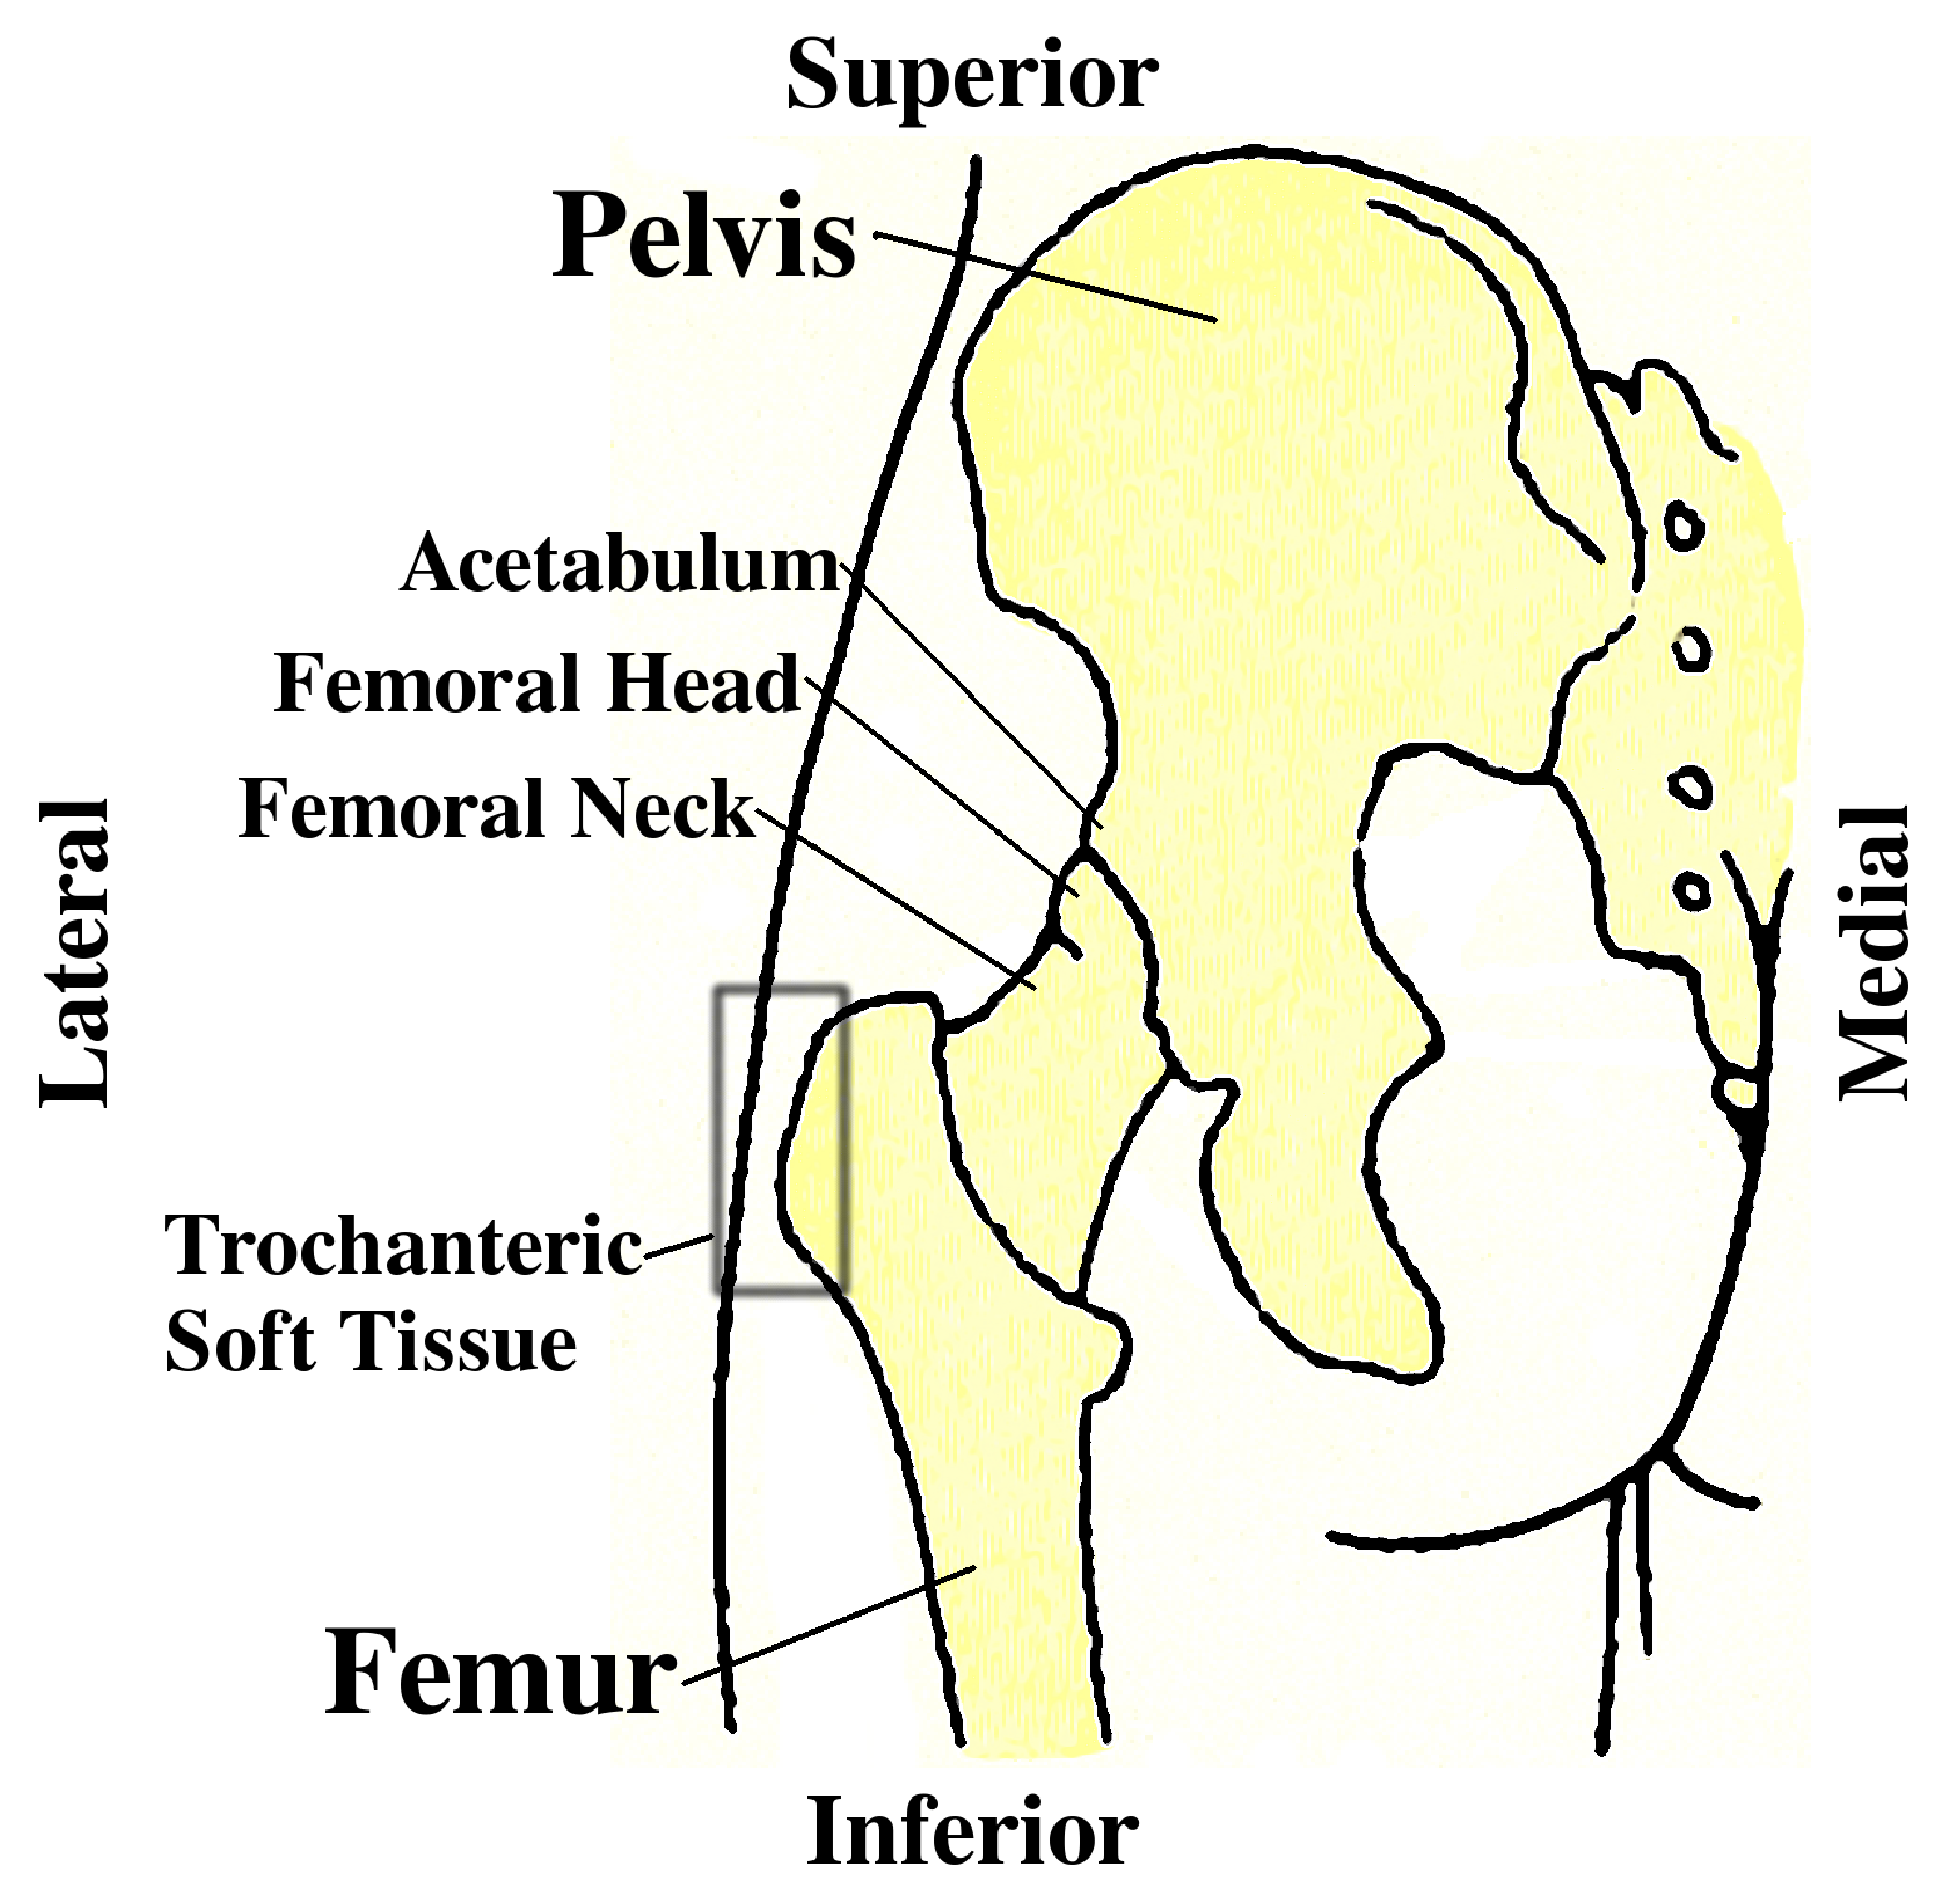
\includegraphics[width=\hsize]{./intro/Figures/Hip_Grays}
\caption[The hip joint]{\textbf{The hip joint is the junction of the trunk with the lower limb. This posterior view shows the pelvis on the medial side with the proximal femur on the lateral side of the joint.} Graphic adapted from~\citet{gray_anatomy_1918} (copyright expired).}
\label{fig:Hip}
\end{figure}

\subsection{Femoral anatomy}
\label{sec:intro_hipAnat_femur}
The femur is a large bone that is crucial for locomotion.
It has many muscle attachments and bony landmarks associated with those attachments.
The largest bony landmarks on the proximal end of the femur are the \textit{greater} and \textit{lesser trochanters} (Figure~\ref{fig:Femur}).
The region between these two landmarks is called the \textit{intertrochanteric region} and is relevant clinically as the site of approximately half of hip fractures~\citep{michelson_epidemiology_1995, lyritis_epidemiology_1996, sirois_burden_2009, lefaivre_changes_2011, poole_cortical_2012}.
The intertrochanteric region has a different morphology on the anterior and posterior aspects.
On the anterior side of the intertrochanteric region is the intertrochanteric \textit{line}, which runs from the supero-lateral greater trochanter to the lesser trochanter. On the posterior side is the intertrochanteric \textit{crest}, which has a similar path to the intertrochanteric line, running from the superio-lateral grater trochanter to the lesser trochanter.
The intertrochanteric crest is more prominent than the intertrochanteric line.

\begin{figure}
\centering
\includegraphics[height=.6\textheight]{./intro/Figures/Femur}
\caption[The femur]{\textbf{The femur, anterior (left) and posterior (right). The trochanters, linea aspera and epicondyles are the insertions of the muscles of the hip and knee joints.} Graphic \textcopyright Seth Gilchrist, 2013.}
\label{fig:Femur}
\end{figure}

Along the posterior aspect of the femoral shaft is the \textit{linea aspera}, which is the insertion for a number of muscles of both the knee and the hip joints.
There are a number of landmarks on the distal end of the femur, but the important ones for the current discussion are the \textit{condyles} and \textit{epicondyles}, which are used to define the coordinate system of the femur.
The condyles of the femur are the weight bearing portions of the distal femur.
The posterior and inferior condyles are approximately aligned with the coronal and transverse planes of the body, respectively in the anatomical position (Figure~\ref{fig:Planes_body}).
The epicondyles of the femur are associated with the colateral ligaments of the knee and are approximately aligned with the coronal plane of the body.

The coordinate system of the femur consists of two anatomical planes, with the third plane defined as orthogonal to the others (Figure~\ref{fig:Planes})~\citep{gray_anatomy_1918}.
The primary plane of reference is the \textit{femoral plane}, which is determined by the three most posterior points on the bone, typically the posterior condyles and trochanter, and is roughly parallel to the coronal plane of the body.
This plane can be thought of as the surface of a table when the bone is placed, posterior down, on the table.
Intraoperatively it is sometimes defined using the epicondyles rather than the posterior condyles, but the correlation between the two definitions is high and the difference small, with an average value of~2$^\circ$~\citep{dorr_comparison_2009}.

\begin{figure}
\begin{subfigure}{0.60\linewidth}
	\centering
	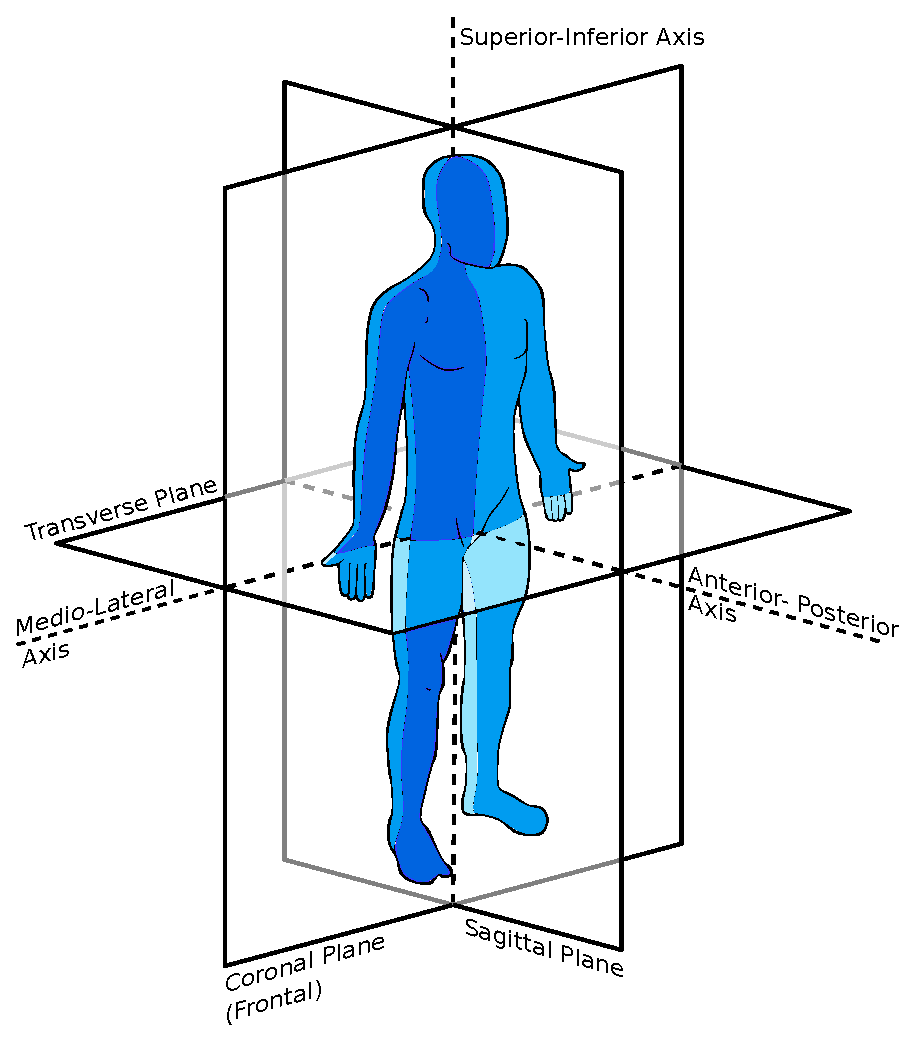
\includegraphics[width=\linewidth]{./intro/Figures/Anatomical-Planes-en}
	\caption{\textbf{Body} Graphic \citet{edoarado_anatomical_2011} (Creative Commons 3.0).}
	\label{fig:Planes_body}
\end{subfigure}
\begin{subfigure}{0.36725\linewidth}
	\centering
	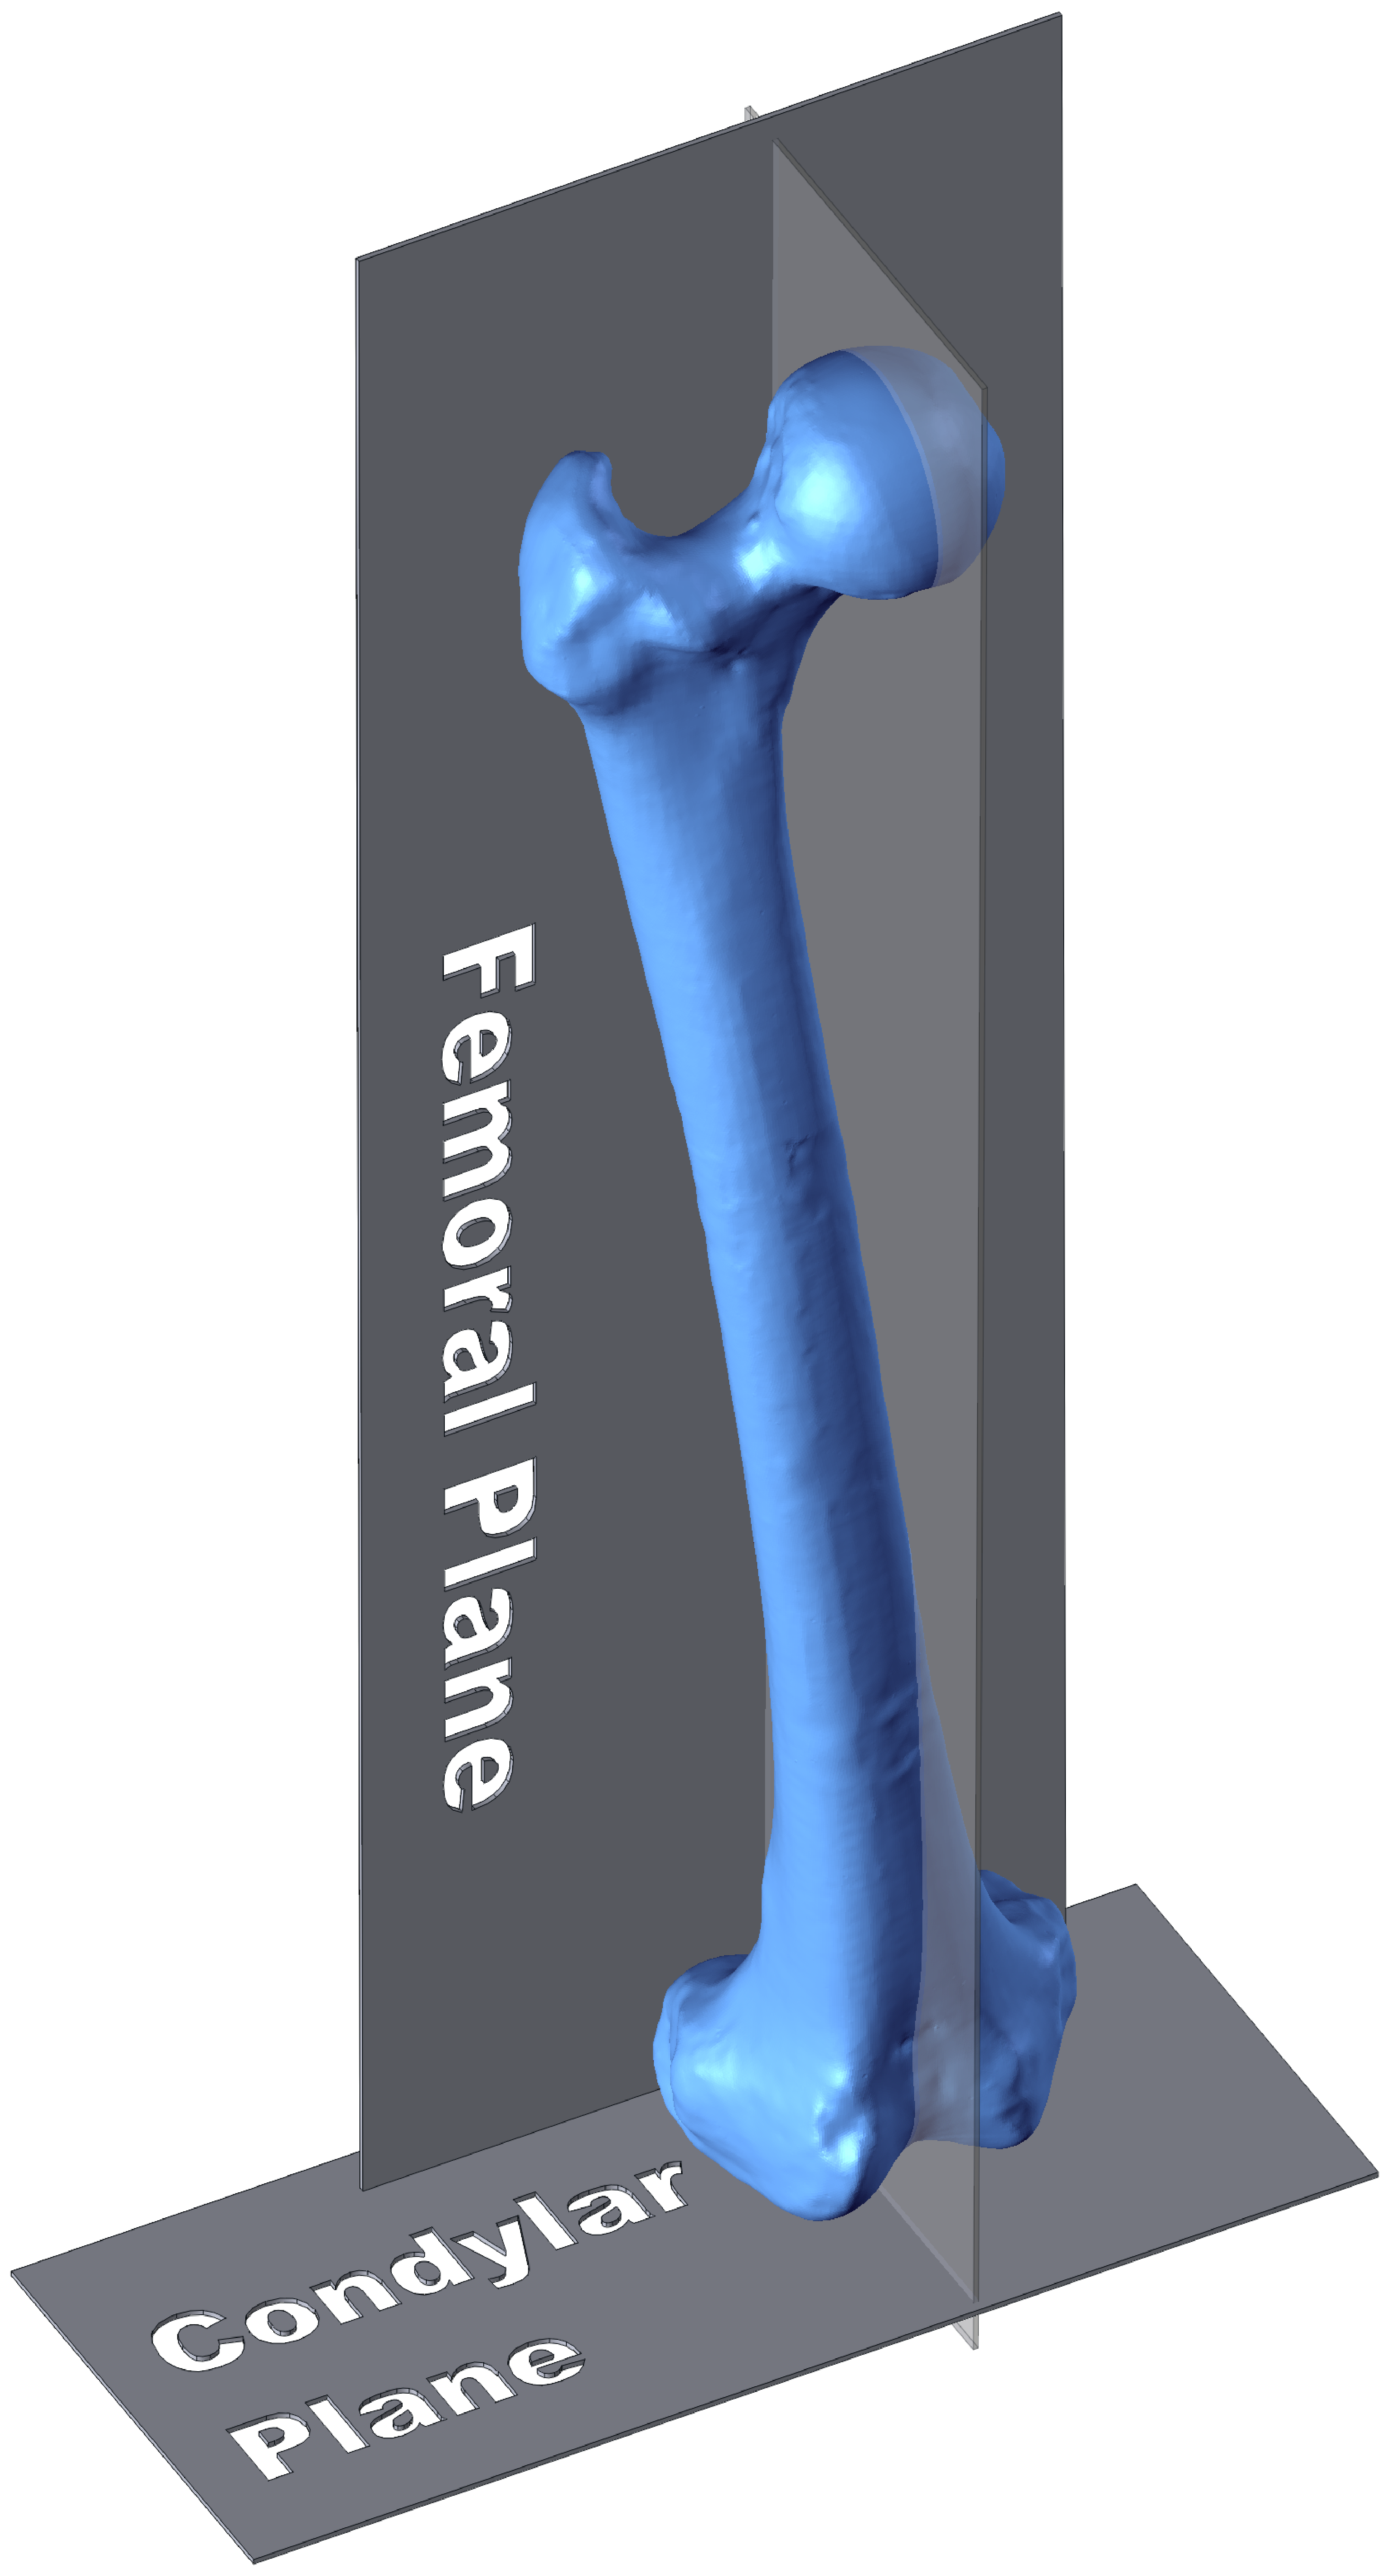
\includegraphics[width=\linewidth]{./intro/Figures/FemoralPlanes}
	\caption{\textbf{Femur} Graphic \textcopyright Seth Gilchrist, 2013.}
	\label{fig:Planes_femur}
\end{subfigure}
\caption[Anatomical and femoral geometrical references]{\textbf{Anatomical planes and directions for the body and femur. In (b), the femoral and condylar planes are labelled, and the mechanical plane is shown with transparency.} }
\label{fig:Planes}
\end{figure}

The second plane is the \textit{condylar plane}, and is defined as perpendicular to the femoral plane, and in contact with the inferior condyles.
It is roughly parallel to the transverse plane of the body.
The \textit{mechanical plane} is defined as perpendicular to the other two planes, passing through the centre of the femoral head, and is approximately parallel to the sagittal plane of the body.
This plane contains the mechanical axis of the femur, running from the centre of the femoral head to the point between the femoral condyles.

The femur has natural curves and twists that occur along its length.
The most obvious curve is the anterior bow of the femur~\cite{gray_anatomy_1918}, which is a bending of the shaft along its length, and occurs predominantly in the third plane.
A more subtle feature is the orientation of the femoral neck to the femoral plane, called \textit{femoral twist} or \textit{femoral version} (Figure~\ref{fig:Version}).
When the neck extends anteriorly to the femoral plane the bone is said to be anteverted, and if it extends posteriorly to the femoral plane it is said to be retroverted.
The femoral version can be measured in a number of different ways using different aspects of the neck to define its orientation.
Using the transverse mid-point of the lateral femoral neck and the centre of the femoral head is called the Kingsley-Olmsted method~\citep{kingsley_study_1948}, considered the clinical standard for version definition.
Other methods of measurement particular to modern imaging systems have also been devised, one example being the use of the anterior surface of the femoral neck as observed using ultrasound~\citep{aamodt_femoral_1995}.
Using the Kingsley-Olmsted method, the normal population has an anteversion angle of (mean(SD)) 9.73$^\circ$(9.82$^\circ$)~\citep{toogood_proximal_2009}.

\thisfloatsetup{floatwidth=0.5\textwidth,capbesidewidth=sidefil,capposition=beside,capbesideposition={top,right}}
\begin{figure}
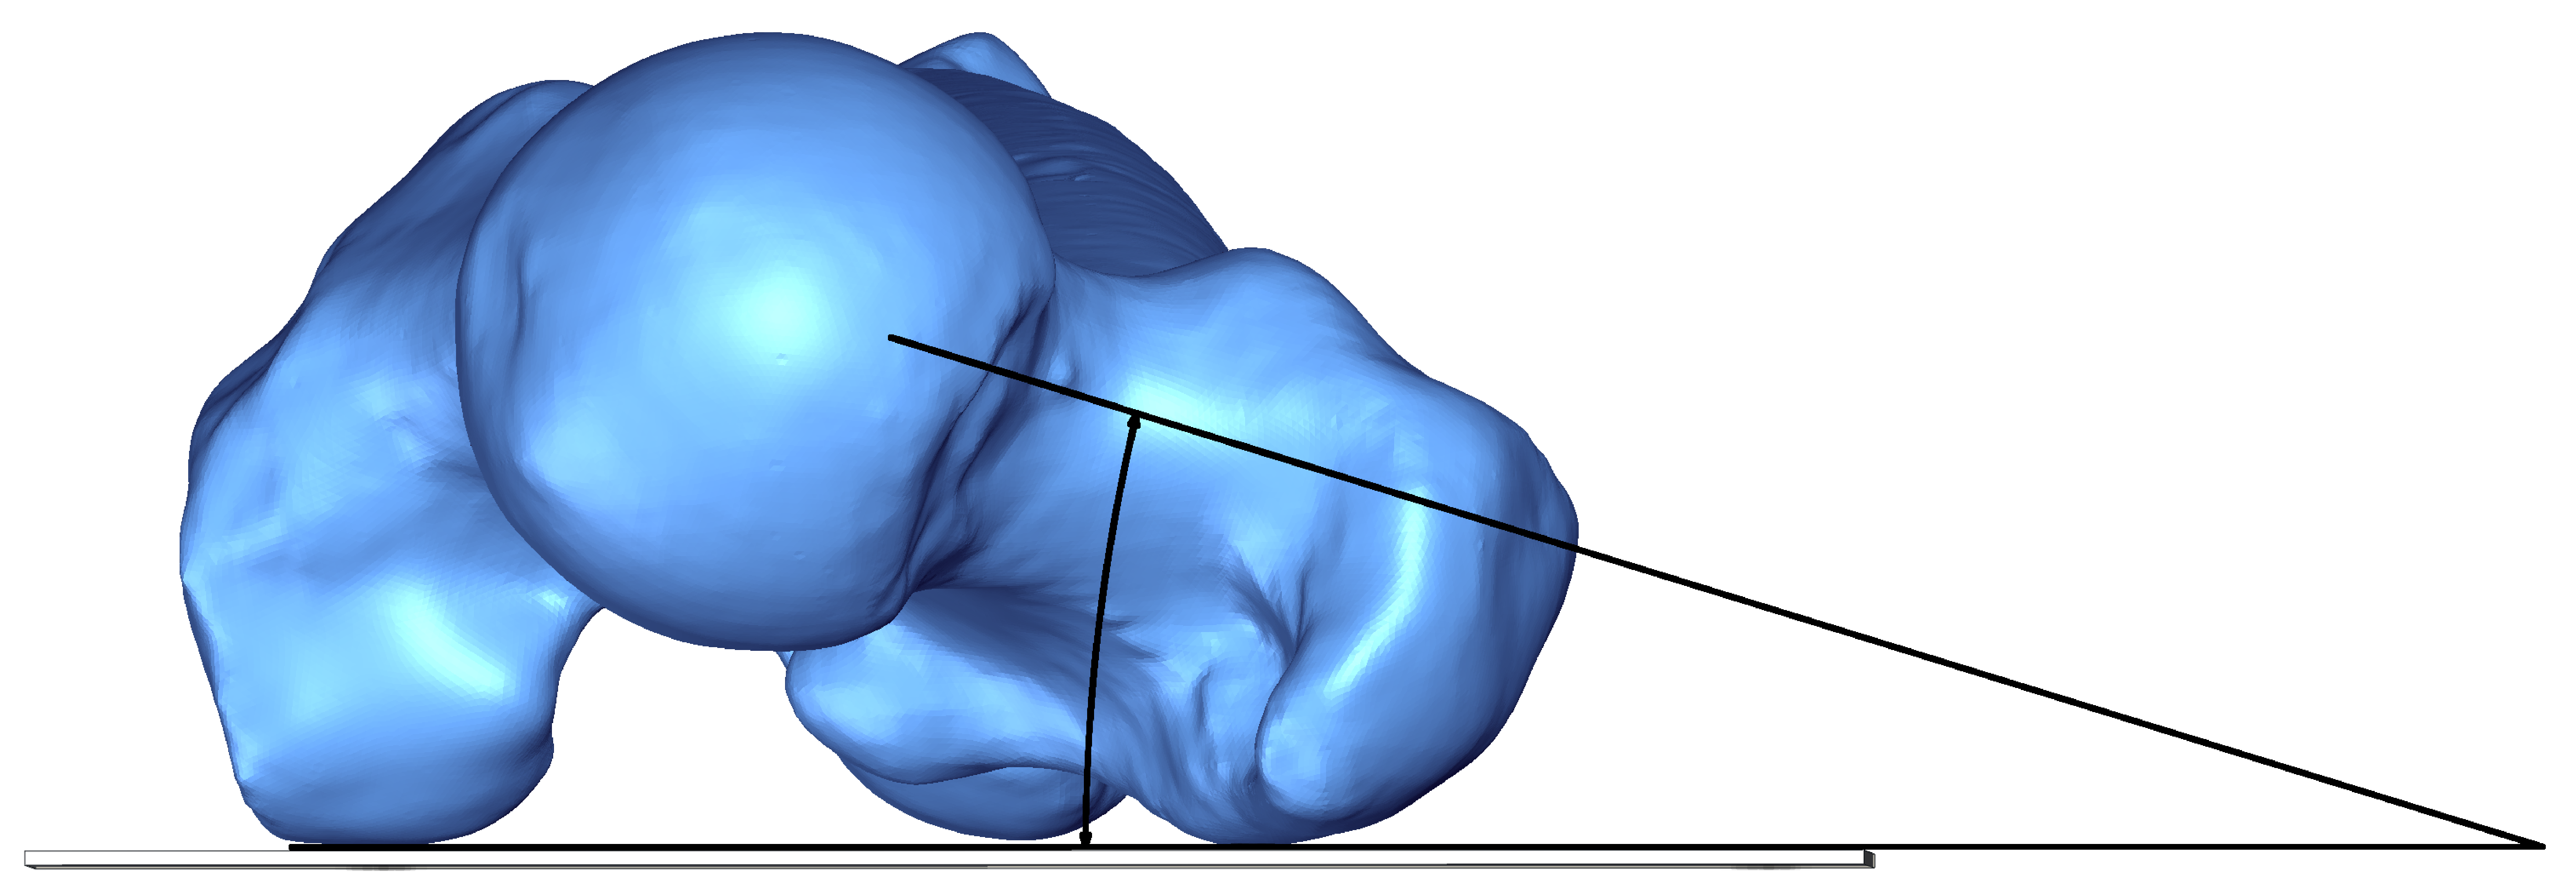
\includegraphics[width=\hsize]{./intro/Figures/Version}			
\caption[Femoral version]{\textbf{Femoral version is the acute angle between the neck and the femoral plane. It is measured by observing the angle from the superior aspect. This images shows the neck axis as defined using the Kingsley-Olmsted method~\cite{kingsley_study_1948}, where the midpoint of the lateral femoral neck is identified from the supero-lateral aspect and is connected to the centre of the femoral head. This specimen is anteverted by an angle of 15.2$^\circ$.} Image \textcopyright Seth Gilchrist, 2013.} 
\label{fig:Version}
\end{figure}

\subsection{Bone anatomy}
\label{sec:intro_boneAnat}
The bones of the body are important organs, with roles in support and movement as well as physiological homoeostasis.
They are composite structures with material types and properties that very spatially and in time.

At a material level, bone is made up of a collagen mesh that is mineralized by hydroxyapatite, and organized in a laminar fashion, making it strong and stiff.
At a structural level bone is classified into two types: cortical and cancellous (Figure~\ref{fig:bone_cancellous}).
Cortical bone (\acs{aka} compact bone) is primarily found in the shaft (or diaphysis) of long bones, and also makes up the exterior shell of irregular bones.
Cancellous bone (\acs{aka} spongy, or trabecular bone) is a low density network, consisting of columns and plates of bone that form a cellular solid.
It is found in the ends (or epiphyses) of long bones, and in the interior of most irregular bones.

\begin{figure}
\begin{subfigure}{0.49\linewidth}
	\centering
	\includegraphics[width=\linewidth]{./intro/Figures/Ascenzi_proximal}
\end{subfigure}
\begin{subfigure}{.49\linewidth}
	\centering
	\includegraphics[width=\linewidth]{./intro/Figures/Ascenzi_trabec}
\end{subfigure}
\caption[Cortical and cancellous bone images in the proximal femur]{\textbf{Left: A section of the proximal femur. Cortical bone serves as the exterior envelope of the organ, with cancellous bone in the interior. Right: Close up view of the cancellous bone showing plate-like (A) and rod-like (B) trabeculae.} Images adapted from~\citet{ascenzi_variation_2011} (with permission).}
\label{fig:bone_cancellous}
\end{figure}

There are two types of cortical bone, with names that refer to the organization of the collagen network: woven and lamellar.
\textit{Woven} bone is characterized by an unorganized, tangle of collagen Type-I fibres, and is mechanically weak.
In adults, woven bone is transient, created after injury where quick reinforcement is needed, and replaced by lamellar bone as healing progresses.

\textit{Lamellar} bone is characterized by long, laminarly organized, mineralized, collagen Type-I fibres.
Two subtypes of lamellar bone are commonly found in the appendicular skeleton: osteonal and interstitial.
Osteonal lamellar bone is contained within osteons (also called Haversian systems) which are concentric rings of lamellar bone that surround a central nutrient-transport canal (Figure \ref{fig:Compact_bone}).
The collagen fibres in the bone of the Haversian systems are oriented in roughly the same direction, but can be as much as 90$^\circ$ off from adjacent layers (both running 45$^\circ$ from the osteon axis).
Interstitial lamellar bone consists of fragments of lamellar bone that fill the gaps between Haversian systems.

\thisfloatsetup{floatwidth=0.5\textwidth,capbesidewidth=sidefil,capposition=beside,capbesideposition={top,left}}
\begin{figure}
\includegraphics[width=\hsize]{./intro/Figures/Compact_bone}			
\caption[Cortical bone cross-section]{\textbf{A cross-section of cortical bone at high resolution. The concentric rings are lamellar bone (each about 5~\ac{micro-m} thick), organized into Haversian systems. The spaces between the Haversian systems contain interstitial lamellar bone.}. Image courtesy of~\citet{konrad_compact_2009} (public domain).}
\label{fig:Compact_bone}
\end{figure}

Cortical bone is quantified using either density (\acs{g}/\acs{cm}$^3$), or \acf{bv/tv} in conjunction with beam section properties such as the second area moment of inertia.

Cancellous bone is also made up of lamellar bone; however, the mesioscale (\acs{ie}, between micro- and macroscale) organization of cancellous bone gives it significantly different structural properties.
It has an open cell structure that is made up of discrete rod- and plate-like trabecular elements (Figure \ref{fig:bone_cancellous}).
This structure means that cancellous bone is much softer and better at absorbing energy than cortical bone.
The organization of the cellular matrix is critical to the behaviour of the material, and quantification of this structure is done in a number of ways (Table \ref{tab:cancellous}).

% % Define a new command to allow for multiple rows in one cell
% command def from http://tex.stackexchange.com/questions/83757/aligning-text-in-a-table
\newcommand{\lbCell}[2][c]
{ 
\begin{tabular}[#1]{ c }
	#2
\end{tabular}
}

\begin{table}
\footnotesize
\centering
\caption[Trabecular quantification]{Trabecular quantification measures. Many more that have been proposed, but these are the most common.}
\label{tab:cancellous}
\begin{tabular}{l c c m{7cm}}
\toprule
Quantity & Measure  & Units & Description \\
\midrule
Density 	& \lbCell{Bone Volume Ratio \\ (\acs{bv/tv} or V$_V$)} 		& $\frac{mm^3}{mm^3}$  & Ratio of bone volume to total volume in a given \ac{roi}.\\ \hline
Surface Area& \lbCell{Surface Volume Ratio \\  (\acs{bs/tv} or S$_V$)}	& $\frac{mm^2}{mm^3}$ & Ratio of bone surface area to total volume in a given \ac{roi}.\\  \hline
\multirow{2}{2cm}{Trabecular Dimensions}
		& \lbCell{Trabecular Thickness \\ (\acs{tbth})}	& $mm$ & Average trabecular thickness calculated in a random, \ac{2d} slice. \\[1EX] 
			& \lbCell{Trabecular Spacing \\ (\acs{tbsp})} 	& $mm$ & A measure of spacing between trabeculae, derived using a parallel-plate, theoretical model of trabecular morphology. \\ \hline
Anisotropy & \lbCell{Mean Intercept Length \\ (\acs{mil})}	& $mm$ & A measure of the material fabric orientation, derived from \ac{2d} sections, which indicates the number of intersections along a projection from a randomly selected point. Provides a tensor, with the first and third Eigenvectors indicating the maximum and minimum material directions.\\ \hline
\multirow{3}{*}{Topology}
		& \lbCell{Trabecular Number \\ (\acs{tbn})} 		& $\frac{1}{mm}$ & A measure indicating the number of trabeculae in a given volume. Derived using a parallel-plate, theoretical model of trabecular morphology.\\
		& \lbCell{Connective Density \\ (\acs{connd})}	& $\frac{1}{mm}$ & A measure of the number of trabecular intersections. \\
		& \lbCell{Structure Model Index \\ (\acs{smi})}	& unitless  & A measure of morphology as more rod or plate like. An ideal rod structure has an \acs{smi} of 0 and an ideal plate structure has an \acs{smi} of 3.\\
\bottomrule
\end{tabular}
\end{table}

An especially important cancellous bone measurement for the current discussion is the \ac{mil}, which quantifies the orientation of the trabecular network and is important when evaluating material anisotropy.
The \ac{mil} is determined from \ac{2d} sections on which lines at various angles are drawn. The average distances between trabeculae on the lines are recorded at each angle (Figure~\ref{fig:Odgaard_MIL}).
This measurement yields a tensor which defines the fabric properties in any given cut of the bone.
The Eigenvectors and Eigenvalues of the tensor can then be used to determine the principal directions, in much the same way that principal stresses can be determined from the Eigenvectors and values of a stress tensor (Figure~\ref{fig:Eigenvectors}).

\thisfloatsetup{floatwidth=0.5\textwidth,capbesidewidth=sidefil,capposition=beside,capbesideposition={top,right}}
\begin{figure}
\includegraphics[width=\hsize]{./intro/Figures/Odgaard_MIL}
\caption[Determination of \acs*{mil}]{\textbf{A bone cross-section showing the lines used to determine the \acs{mil}. The average distance between the trabeculea along the lines is recorded at various values of the angle $\omega$. An image slice in a perpendicular direction will give the \ac{mil} in the out-of-image dimension.} Graphic adapted from \citet{odgaard_three-dimensional_1997} (with permission).}
\label{fig:Odgaard_MIL}
\end{figure}

\thisfloatsetup{floatwidth=0.5\textwidth,capbesidewidth=sidefil,capposition=beside,capbesideposition={top,left}}
\begin{figure}
\includegraphics[width=\hsize]{./intro/Figures/Ascenzi_trabec_eigenvectors}
\caption[\acs*{mil} of a \acs*{2d} section]{\textbf{Eigenvectors are a mathematical tool for identifying important directions in systems described by tensors. In the case of fabric tensors, like those used for \ac{mil}, the first Eigenvector will point in the direction where most of the bone is oriented. The second and third Eigenvectors will be perpendicular to the first (and each other) and will point in the directions of the other two main material directions. In this \acs{2d} depiction, the first Eigenvector points along the strongest trabeculae and the second points in the perpendicular direction, along transverse supports.} Image adapted from~\citet{ascenzi_variation_2011} (with permission).}
\label{fig:Eigenvectors}
\end{figure}

\section{Fractures of the proximal femur}
\label{sec:intro_fractures}
Fractures of the proximal femur are an important social and clinical problem in Canada and around the world.
They constitute a large proportion of all orthopaedic injuries, with some studies reporting more than 20\% of orthopaedic beds being occupied by hip fracture patients at any given time~\citep{torgerson_letter:_2000}.
While research has shown a trend of decreasing fracture rates in recent years~\citep{lefaivre_changes_2011}, the total incidents of fracture is increasing as the population ages~\citep{wiktorowicz_economic_2001}, and the hospital admissions are becoming more complex, with increasing number of comorbidities~\citep{sirois_burden_2009}.

Fractures are thought to be caused in two ways.
The first, and likely the most common, is as a result of a fall to the side; the second, and less common, is a spontaneous fracture due to extreme bone fragility.
While both types of fractures are important, the focus of the current work is on fractures due to falls as they are thought to constitute upwards of 95\% of hip fracture cases~\citep{parkkari_majority_1999}.

The financial impact of the fractures on the health care system is difficult to overstate.
The 1-year cost of an individual fracture in Canada has been put in the range of CDN\$29,065 -- \$60,013 (\citep{wiktorowicz_economic_2001}, corrected to 2013 dollars by the Bank of Canada~\citep{bank_of_canada_inflation_2013}).
Lifetime costs of a single hip fracture in the US are as high as US\$107,193 (\citep{braithwaite_estimating_2003}, corrected to 2013 dollars by the US Bureau of Labor Statistics~\citep{bureau_of_labor_statistics_cpi_2013}).
All together, these fractures cost the Canadian system CDN\$659M/year (\citep{tarride_burden_2012}, corrected to 2013 dollars by the Bank of Canada~\citep{bank_of_canada_inflation_2013}), and this value could more than double by 2040~\citep{wiktorowicz_economic_2001}.

Considerable work has been performed by the research community to understand and prevent hip fractures.
This section will describe the clinical procedures and burdens of hip fracture, and the research that has been conducted to reduce that burden.

\subsection{Clinical considerations}
\label{sec:fractures_clinic}
Hip fracture is a significant clinical problem, and an understanding of the needs and requirements of the clinical situation is key to developing a meaningful treatment or mitigation strategy.
Clinical interventions begin with screening and, if indicated, continue with prophylactic prescription of either drugs or biomechanical devices, such as hip protectors.
If screening and prevention fail, and a hip fracture results, the most common clinical treatment is surgical repair using plates, screws or full joint components.
There are a variety of surgical options depending on the details of the fracture.

\subsubsection{Early risk assessment}
\label{sec:fractures_clinic_risk}
The primary risk factors for hip fracture are age, falling, and bone density~\citep{cummings_risk_1995}.
Risk assessment and clinical treatment targets are therefore geared towards assessing and addressing these factors.
There are a number of preventative interventions that have shown some success, such as pharmacological~\citep{hodsman_bisphosphonates_2002}, lifestyle~\citep{moayyeri_association_2008} and to some degree hip protectors~\citep{haines_hip_2006}.
The first step to implementing one of these possible treatments is identification of individuals at risk of hip fracture through screening.
The gold standard screening technique is \acf{dxa} to quantify \acf{bmd}, which is then used to evaluate osteoporosis state.

Osteoporosis is a clinical diagnosis of low \ac{bmd}.
It is not a disease in itself, but a condition caused by a number of possible aliments, including vitamin-D deficiency, hormone deficiency, or physiological ageing~\citep[Ch.12]{avioli_metabolic_1998}.
Two metrics exist for rating an individual's bone density.
The \textit{T-score} shows where an individual's \ac{bmd} falls in comparison to a sex and race match young adult population (Equation \ref{equ:tscore}), and the \textit{Z-score} shows where an individual's bone density falls in relation to a sex, race and age-matched population (Equation \ref{equ:zscore})~\citep{orwoll_osteoporosis_2011}.
The definition of osteoporosis state, as given by the \ac{who}, uses the T-score (Table \ref{tab:op}).

\begin{eqnarray}
	\label{equ:tscore}
	T &=& \frac{BMD_{patent} - \overline{BMD}_{lifetime\; peak}}{\acs*{sd}_{lifetime\; peak}} \\ [1em]
	\label{equ:zscore}
	Z &=& \frac{BMD_{patent} - \overline{BMD}_{age-matched}}{\acs*{sd}_{age-matched}}
\end{eqnarray}

\begin{table}
	\caption[\acs*{who} osteoporosis definitions]{\acs*{who} definition of osteoporosis state~\citep{who_study_group_assessment_1994}.}		
	\label{tab:op}
	\begin{tabularx}{0.9\textwidth}{l X}
		\toprule
		\textbf{Classification} & \textbf{Description} \\ \midrule
		Normal                  &  \ac{bmd} greater than 1~\acs{sd} below the young adult average ($T > -1$). \\
		Osteopenia              &  \ac{bmd} between 1 and 2.5~\acs{sd} below the young adult average ($-1 \geq T > -2.5 $).\\
		Osteoporosis            &  \ac{bmd} less than 2.5~\acs{sd} below the young adult average ($T \leq -2.5$).\\ \bottomrule
	\end{tabularx} 
\end{table}

\ac{dxa} is an x-ray imaging technique that provides a measure of mineralized bone content between the x-ray source and collector.
Since a \ac{2d} image is created, the output of the technique is commonly called the \ac{abmd}, in which the \ac{bmc} is normalized by the projected area, and is quantified in units of~$\acs{g}/\ac{cm}^2$.
To measure \ac{bmc}, the \ac{dxa} method breaks the human body into two components: soft tissue and bone mineral.
The soft tissues of the body all have approximately the same x-ray attenuation, which is significantly lower than that of bone mineral.
With only two components, the amount of each can be found by simultaneously solving the Beer-Lambert relation at two energy levels (Equations~\ref{equ:dxa1} and~\ref{equ:dxa2})~\citep{jacobson_x-ray_1964, gustafsson_x_1974}.

\begingroup
\setlength{\abovedisplayskip}{-2ex}
\begin{eqnarray}
\label{equ:dxa1}
	I_1 = I_{0,1} \cdot e^{-(\mu_{1,t} \cdot x_t + \mu_{1,b} \cdot x_b)} \\ [1ex]
\label{equ:dxa2}
	I_2 = I_{0,2} \cdot e^{-(\mu_{2,t} \cdot x_t + \mu_{2,b} \cdot x_b)} 
\end{eqnarray}
\endgroup

\acused{n/eng} \acused{i/eng} \acused{mu/attn} \acused{x/dxa} \acused{t/dxa} \acused{b/dxa} % acronyms that are spelled out below

\ac{i/eng}$_{0,n}$ and \ac{i/eng}$_n$ are the incident and transmitted x-ray intensities at energy level $\ac{n/eng}$, respectively.
\ac{mu/attn}$_{n,t}$ and \ac{mu/attn}$_{n,b}$ are the linear attenuation coefficients at energy level \ac{n/eng} for the \acf{t/dxa} and \acf{b/dxa}, and \ac{x/dxa}$_t$ and \ac{x/dxa}$_b$ are the path lengths in the \acl{t/dxa} and \acl{b/dxa}.
The transmitted and incident energy levels, as well as the absorption coefficients, are known \textit{a priori}, and therefore the path lengths can be solved.
The product of the known density of bone mineral ([\ac{kg}/\ac{m}$^3$]) with the calculated path length ([\ac{m}]) is \ac{abmd} ([\ac{kg}/\ac{m}$^2$]).

Modern \ac{dxa} machines include internal calibrations of known path lengths to ensure accuracy~\citep{guillemot_pelvic_1997}; however, there are a number of issues that must be considered when calculating \ac{abmd} using \ac{dxa}~\citep{bolotin_patient-specific_2003}.
To begin with, data from \ac{dxa} machines cannot be readily compared across manufacturers~\citep{genant_universal_1994}.
Each manufacturer creates a custom database of population \acp{abmd}, making it possible to compare T- and Z-scores. However, direct comparison of \ac{abmd} values must be corrected based on a standard calibration performed on each machine~\citep{genant_universal_1994}.

Secondly, the changes in bone quality can happen in either the cancellous or cortical compartments.
Cancellous bone, by its very nature, has a lower projected density than cortical bone, and therefore makes up a smaller portion of the $x_b$ in Equations \ref{equ:dxa1} and \ref{equ:dxa2}.
In the early stages of bone loss, cancellous bone changes can be more pronounced than cortical bone changes, but may not be detected by \ac{dxa} screening~\citep{guglielmi_osteoporosis:_1994}.

Third, spurious calcification of the bones and/or adjacent structures can interfere with \ac{dxa} measurements.
Osteophytes (calcification of bone in non-load-bearing regions) are common in the elderly~\citep{rand_impact_1997}, and have a significant effect on \ac{abmd} readings~\citep{rand_impact_1997}.
Adjacent structures can be ossified ligaments and cartilage or calcium deposits in the aorta, which runs adjacent to the spine~\citep{smith_aortic_1999}.
Calcification of these structures will increase the derived \ac{abmd} and lead to an inappropriate osteoporosis classification.

The final problem is caused by projection issues due to the size of the bone being scanned, versus the average size of the bone in the reference population.
In the projection of an object, the volume increases faster than its projected area as its characteristic length increases.
This can lead to bones that are significantly larger than the reference population having higher \ac{abmd}, which may be mistaken for higher \ac{bmc}~(see \S\ref{sec:support_abmd} for an example calculation).

In order to address some of these limitations, the \ac{who} developed the \ac{frax} which can be used either in conjunction with \ac{bmd} measurements, or as an independent analysis~\citep{kanis_fraxtm_2008}.
The \ac{frax} score is based on twelve risk factors and provides a 10~year probability of spine, humerus or wrist fracture, as well as a 10~year probability of hip fracture (Table~\ref{tab:frax}).

\begin{table}
\caption[Inputs to the \acs*{frax} model]{Inputs into the \acs*{frax} model. The inclusion of \ac{bmd} is optional~\citep{kanis_fraxtm_2008, van_den_bergh_assessment_2010}.}
\label{tab:frax}
\begin{tabularx}{0.75\textwidth}{>{\centering\arraybackslash}X >{\centering\arraybackslash}X}
\toprule
\textbf{Risk Factor} & \textbf{Data} \\ 
\midrule
 Age & Years \\ 
 Gender & Male or Female \\ 
 Weight & \ac{kg} \\ 
 Height & \ac{cm} \\ 
 Previous Fracture & Yes or No \\ 
 Parent Fractured Hip & Yes or No \\ 
 Current Smoking & Yes or No \\ 
 Glucocorticoids & Yes or No \\ 
 Rheumatoid Arthritis & Yes or No \\ 
 Secondary Osteoporosis & Yes or No \\ 
 Alcohol $\geq$3 units per day & Yes or No \\ 
 Femoral Neck \ac{bmd} & T-score or Z-score \\ 
\bottomrule 
\end{tabularx} 
\end{table}

The \ac{frax} tool must be calibrated for each population for which it is used, as the weighting of each risk factor cannot be generalized.
Once it has been calibrated, \ac{frax} can help identify those at risk of fracture.
The efficacy of the tool is dependent on the probability cutoffs used.
For example, if a 10~year fracture probability of 20\% is used as a cutoff, nearly 30\% of those who will suffer a fracture can be identified~\cite{leslie_fracture_2011}.
While identification of 30\% of individuals is high, it is only moderately higher than the 28\% that can be identified by osteoporosis score alone~\citep{stone_bmd_2003}, and has been shown to be no better than using only \ac{bmd} + age and neglecting the other ten risk factors~\citep{van_den_bergh_assessment_2010}.
A major strength of the \ac{frax} tool is that an initial assessment can be conducted without the need for a \ac{dxa} scan, and if the individual is found to be in an intermediate risk group, a \ac{dxa} scan can be performed and the person's risk level re-evaluated~\citep{kanis_frax_2009}.

Keeping these limitations in mind, \ac{frax} and \ac{dxa} provide simple, fast and useful clinical tools.
\ac{dxa} provides a single number (in the case of \ac{abmd}) or designation (in the case of osteoporosis state) that indicates a clinical course of action.
\ac{frax} can be used as a pre-screening tool for \ac{dxa} scanning and can refine the individual risk if \ac{dxa} scanning is indicated.
The \ac{who} recommends screening women over the age of 65, which is a significant screening burden, and while uptake is high, it is not 100\%~\citep[p.~101]{who_study_group_assessment_1994}.
The \ac{who} also recognizes the fact that many individuals who are screened using these tools and found to be free from osteoporosis will still go on to fracture~\citep[p.~99]{who_study_group_assessment_1994}.
		
\subsubsection{When screening fails}
\label{sec:fractures_clinic_fail}
Even for those who undergo screening, falls cannot always be avoided, and hip fracture cannot always be prevented.
Depending on the fracture type, location, and any comorbidities, there are a number of treatment options available to clinicians -- most of them surgical.

Patients that present with hip fracture due to fagility are typically older and female~\citep{cummings_epidemiology_2002}.
After initial assessment has indicated a possible hip fracture, anterior-posterior x-rays of the hip are used to classify of the fracture type, which guides treatment.

Fracture classification is hierarchical and helps to indicate the appropriate intervention.
The highest level is intracapsular vs.\ extracapsular fracture, which references the fracture location in terms of whether it is located inside or outside the joint capsule (Figure~\ref{fig:HipCapsule}).
Intracapsular fractures are fractures of the femoral neck and are further classified into basicervical, cervical or subcapital fractures (Figure \ref{fig:NeckFractues}).
Basicervical fractures occur in the femoral neck, at the junction with the trochanter; cervical fractures occur somewhere along the length of the neck; and subcapital fractures occur at the base of the femoral head.

\begin{figure}
\centering
\includegraphics[width=0.7\linewidth]{./intro/Figures/HipCapsule}
\caption[The hip joint capsule]{\textbf{Posterior view of the hip showing the hip joint capsule. The capsule comprises the blue membrane, which has been distended in this view for visualization.} Graphic adapted from~\citet{gray_anatomy_1918} (copyright expired).}
\label{fig:HipCapsule}
\end{figure}

Extracapsular fractures are sub-classified into intertrochanteric, trochanteric, or subtrochanteric (Figure~\ref{fig:ExtracapFractues}).
Intertrochanteric (\acs{aka} pertrochanteric) fractures run between the greater and lesser trochanters, just lateral to the line of a basicervical fracture; trochanteric fractures involve only one of the trochanters; and subtrochanteric fractures involve the femoral diaphysis, distal to the lesser trochanter. 
The proportions of each fracture type are roughly 45\% intracapsular, 55\% extracapsular; however, that ratio seems to be changing, with a tendency to fewer intracapsular fractures~\citep{haleem_mortality_2008}.

\begin{figure}
	\centering
	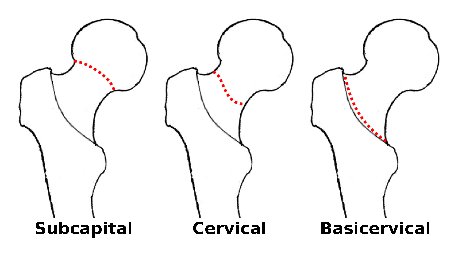
\includegraphics[width=0.7\linewidth]{./intro/Figures/NeckFractues}
	\caption[Intracapsular fractures]{\textbf{Intracapsular fractures of the proximal femur.} Graphic \copyright Seth Gilchrist, 2013.}
	\label{fig:NeckFractues}
\end{figure}

\begin{figure}
	\centering
	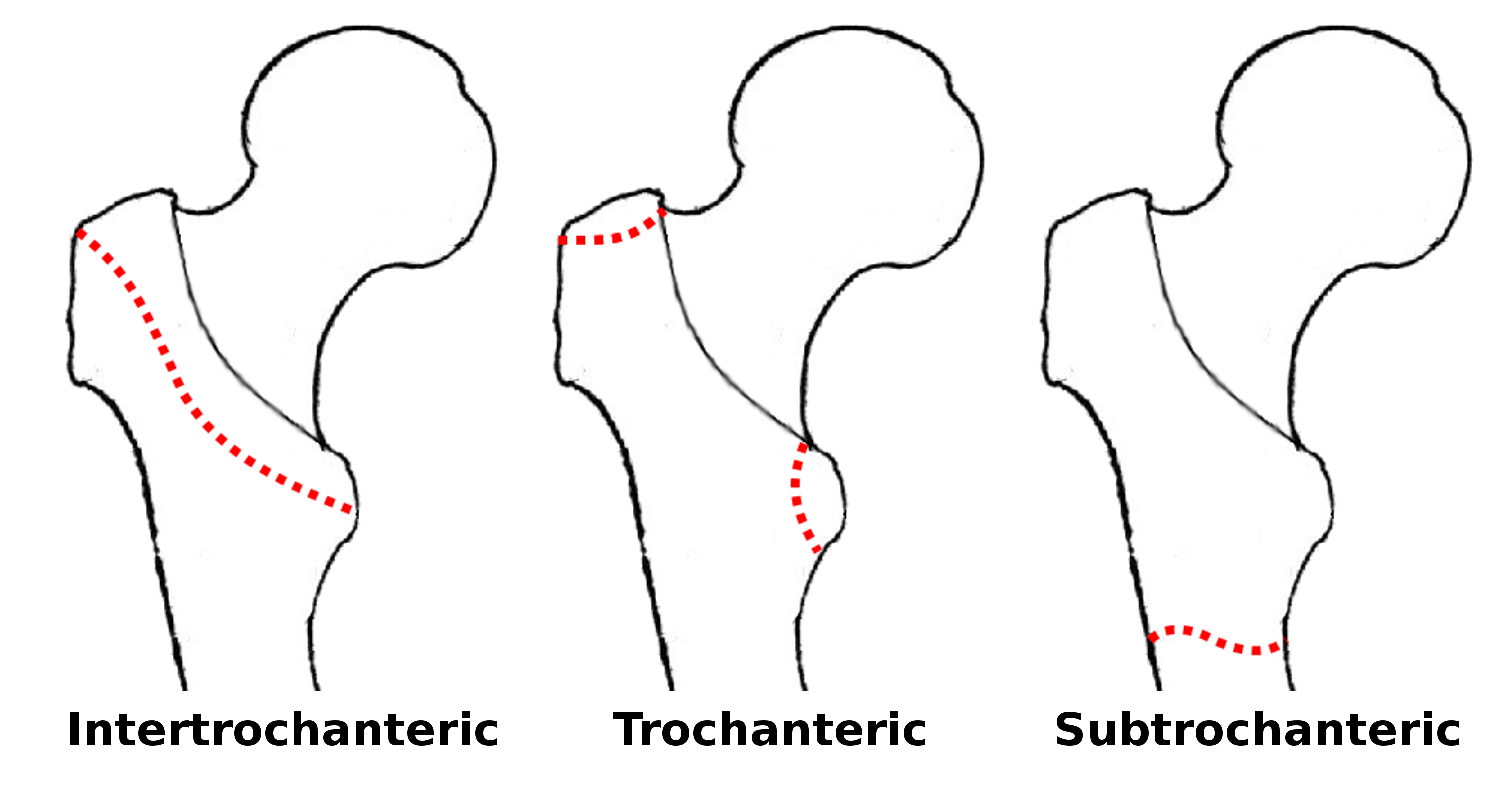
\includegraphics[width=0.7\linewidth]{./intro/Figures/ExtracapFractues}
	\caption[Extracapsular fractures]{\textbf{Extracapsular fractures of the proximal femur.} Graphic \copyright Seth Gilchrist, 2013.}
	\label{fig:ExtracapFractues}
\end{figure}

There are two surgical strategies for hip fracture treatment: repair and replacement.
Surgical repair of proximal femur fractures involves reduction and fixation, while surgigal replacement includes hemiarthroplasty, and \ac{tha}.
Reduction is the process of aligning fractured fragments, which are then secured in place using fixation, typically utilizing plates, rods screws and/or nails.
Reduction can be either \textit{open}, in which the fragments are dissected, and oriented manually, or \textit{closed}, where external pressure and traction are used to align fragments.
\ac{tha} involves resection of the femoral head and neck, reaming of the acetabular cup, and replacement of these components with a stem and ball on the femoral side and an articulating cup on the pelvis side.
In hemiarthoplasty, this procedure is done only on the femoral side and the acetabular anatomy is left in place.

The indications for the type of surgical solution can be quite complex~\citep{simon_emergency_2011, browner_skeletal_2002}.
They rely on the location of the fracture~\citep{bray_femoral_1997, delamora_introduction_2002}, the angle of the fracture line~\citep{bray_femoral_1997}, the age of the patient~\citep{shah_algorithms_2002,bhandari_internal_2003}, time since fracture~\citep{bray_femoral_1997, delamora_introduction_2002}, and any comorbidities~\citep{shah_algorithms_2002, bhandari_internal_2003}.
Depending on the severity and type of comorbidities, surgery may not be an option, in which case non-operative treatment may be required.
Non-operative treatment of hip fracture has shown poor outcomes and is not common~\citep{heim_nonoperative_2002}.
It requires an extended period of non-weight bearing ($\sim$6~weeks), which can exacerbate existing bone quality issues, and has been seen to have poorer long-term outcomes compared to repair or replacement strategies~\citep{heim_nonoperative_2002}.

Hip surgery has a high success rate~\citep{heim_nonoperative_2002, bhandari_internal_2003, browner_skeletal_2002}, and is the preferred treatment option for hip fracture.
That said, hip fracture is a very serious injury and can result in a decrease in quality of life, extended morbidity, and even mortality.
\citet{wiktorowicz_economic_2001} found 38.4\% of community dwelling individuals who suffered hip fractures were discharged into either assisted living (27.1\%), or died (11.3\%).
This is corroborated by another study that found 26\% of community dwelling individuals were discharged to assisted living after hip fracture~\citep{cooper_crippling_1997}.
Additionally, hip fracture patients spend more time in assisted living than age-matched controls -- an average of 237 more days than a typical 80 year old~\citep{braithwaite_estimating_2003}.

Mortality following hip fracture is also high.
While death generally isn't directly attributable to the fracture, hip fracture patients fare much worse than their age-matched controls due to a range of systemic deleterious health effects~\citep{cooper_crippling_1997}. 
In the three months following hip fracture, patients have a mortality \ac{or} of 2.8 over age-matched controls~\citep{richmond_mortality_2003}.
This gradually decreases back to an \ac{or} of 1.4 at two years, but mortality rates remain higher than age-matched controls for at least five years post fracture~\citep{cooper_crippling_1997}.
In actual percentages of patients, one year post fracture, up to 21.6\% of patients have died~\citep{wiktorowicz_economic_2001}.

This section has discussed the clinical screening, treatment and discharge paths of hip fracture patients.
The treatment and discharge sections show just how important screening is.
Research conducted to improve screening efficacy is of clear benefit to patients and society.
Only with accurate screening abilities will we be able to concentrate our prevention efforts -- be they pharmacological, lifestyle or surgical strengthening -- on the most vulnerable people. 

\section{Mechanical behaviour of bone}
\label{sec:intro_boneBehaviour}
Before addressing hip fracture test methods and models, the mechanical behaviour of the materials that comprise the proximal femur need to be understood.
In Section~\ref{sec:intro_hipAnat} I discussed the anatomy of the femur and the bone were discussed.
This section builds on that knowledge by outlining the mechanical behaviours of these materials based on anatomical and morphological differences.
Following this discussion of the mechanical behaviours, the different methods for modelling hip fracture will be discussed, in which the material level behaviours will be important.

The bones of the body are complex organs that are made up of multiple materials serving a variety of functions.
The principal load bearing material is named after the organ itself and is called \textit{bone}.
Bone material is inhomogeneous, anisotropic and viscoelastic.
This means that its mechanical properties vary with location, loading direction, and loading speed.
These facts make determination of bone mechanical properties challenging.

Mechanical characterization of bone is done using traditional materials testing methods in which specimens are formed into regular geometries and stretched, compressed or sheared.
Cortical bone is typically milled into dog-bone specimens for tensile testing, and either cuboidal or cylindrical specimens for compression testing~\citep{currey_effects_1975, reilly_elastic_1975, evans_response_1992}.
In cortical bone, the ``orientation" of the specimen is determined by how the loading axis is aligned with the axis of the predominate Haversian system.
Bone is a linearly elastic material, and as such can be characterized in the elastic loading regime using the modulus of elasticity.
The modulus of elasticity of cortical bone varies depending on the orientation of loading (Table \ref{tab:bone_behave}).
It is highest in the longitudinal direction (aligned with the collagen fibrils), and lowest in the transverse direction.

\begin{table}[t]
\caption[Elastic properties of bone]{Approximate cortical and cancellous bone material properties~\citep{reilly_elastic_1975, lotz_mechanical_1991, rincon-kohli_multi-axial_2009}. Longitudinal is along the principal material direction, which is defined by the Haversian system in cortical bone and the first Eigenvector of the \ac{mil} tensor in cancellous bone. Transverse is perpendicular to the Haversian system in cortical bone, and along the third Eigenvector of the \ac{mil} tensor in cancellous bone.}
\label{tab:bone_behave}
\begin{tabularx}{0.8\textwidth}{l l >{\centering\arraybackslash}X >{\centering\arraybackslash}X }
\toprule
				&					& 	\multicolumn{2}{c}{Bone Type}	\\
Modulus (GPa)	& Direction			& Cortical 			& Cancellous	\\	\midrule
Tensile			& Longitudinal		& 17.9				& 2.0			\\
 				& Transverse		& 10.1 				& 0.2			\\[1EX]
Compressive		& Longitudinal		& 18.2				& 9.5			\\
				& Transverse		& 11.7 				& 5.5			\\[1EX]
Shear 			& Transverse		& 3.5				& 0.017			\\
\bottomrule			
\end{tabularx}
\end{table}

Cancellous bone is typically milled into cuboidal or cylindrical specimens for testing~\citep{helgason_mathematical_2008}, with the orientation often given in a site-specific manner~\citep{carter_compressive_1977, fyhrie_failure_1994, nazarian_densitometric_2007}.
For example, the testing direction for cancellous bone of the femoral neck will be given as parallel or perpendicular to the femoral neck axis.
It is becoming more common to also report the orientation with reference to fabric properties, such as \ac{mil}~\citep{rincon-kohli_multi-axial_2009}.
Using the anatomical reference, longitudinal loading is along the direction of the site-specific principal length (\ac{eg}, along the femoral neck); however, using the fabric properties, longitudinal loading is along the first Eigenvector of the fabric tensor~(Figure~\ref{fig:Eigenvectors}.
Transverse loading is perpendicular to the longitudinal direction.
When used with site-specific reference the term \textit{transverse} does not give any information regarding the direction in the plane perpendicular to the principal length in which the loading is taking place.
For example, transverse loading of a femoral neck specimen would be radial loading of the femoral neck bone; however, the direction of the radial (\ac{eg}, anterior-posterior) would not be given.
When fabric properties are used, researchers will normally give the Eigenvector along which they are loading, rather than using term transverse. For example, a specimen subjected to transverse compression would be loaded along the second or third Eigenvector.

The modulus of elasticity and strength of cancellous bone react to changes in orientation similarly to cortical bone (Table \ref{tab:bone_behave}).
Loading along the first Eigenvector of the \ac{mil} tensor yields the highest modulus and strength.
Loading along the third Eigenvector of the \ac{mil} tensor yields the lowest modulus and strength.
In addition to the material orientation variations, the density of the cancellous bone influences the strength, stiffness and post yield behaviour~\citep{carter_compressive_1977, rincon-kohli_multi-axial_2009}.

Both cortical and cancellous bone have been shown to be viscoelastic, meaning that their material properties change with strain rate.
In both types of bone, stiffness has been shown to increase with strain rate~\citep{crowninshield_response_1974, evans_response_1992, pithioux_comparison_2004, carter_compressive_1977, carter_bone_1976, currey_effects_1975}.
In cortical bone loaded in compression, stress at a fixed strain shows a logarithmic relationship with strain rate~\cite{mcelhaney_dynamic_1966}, following the equation $\sigma_\varepsilon = 4200 \log (\dot{\ac{eps}}) + 33,000$ where \acs{sigma}$_\varepsilon$ is the stress at a given strain, and $\dot{\ac{eps}}$ is the strain rate.
Loaded in tension, the modulus of elasticity of cortical bone shows much less variation, being almost invariant with strain rate up to strain rates of 100\ac{eps}/\ac{s}~\citep{crowninshield_response_1974}.

For cancellous bone in compression, researchers have shown that stiffness follows a power-law relationship with strain rate~\citep{carter_compressive_1977, linde_mechanical_1991}.
In one set of tests, the stiffness of de-fatted cancellous bone was proportional to $ \dot{\ac{eps}}^{0.06} $~\citep{carter_compressive_1977}, and in another it was found to be proportional to $ \dot{\ac{eps}}^{0.047} $~\citep{linde_mechanical_1991}.
Importantly, this relationship broke down when the marrow was left \textit{in situ}.
When compression tests were performed on cancellous bone cores with marrow and fat still present, there was a sharp increase in stiffness at the highest strain rates tested (10/\ac{s})~\citep{carter_compressive_1977}.
There were too few specimens in this group to obtain a good fit, but qualitatively an increase in stiffness of about 3x can be seen in the plots presented by \citet{carter_compressive_1977}.
High-rate tension testing of cancellous bone has never been done, so the nature of the relationship is currently unknown.

Generally speaking, cortical and cancellous bone can be said to be stiffest in compression along their principal directions, weakest in shear, with tension in the middle.
Additional considerations for cancellous bone are that stiffness can vary with density and structure.
Effective measures of bone behaviour will take into account the type of bone, the amount present, its orientation to the loading vector, and the rate of force or strain application.

\section{Determinants of bone strength}
\label{sec:intro_boneStrength}
Bone strength refers to the ability of the material to support a given load.
While this definition may sound simple, examination of the details yields a more nuanced view.
As a multiphase, polymorphic, composite material, bone has the ability to behave in a highly ductile manner, a highly brittle manner, or anywhere in between~\citep{hayes_biomechanics_1997}.
Cortical bone tends to behave in a brittle manner, and as such, ultimate load or stress is often given as the strength of the bone~\citep{hayes_biomechanics_1997, reilly_elastic_1975}.
Cancellous bone is more ductile in its failure modes, and ultimate properties would not tell as complete of a story.
For this reason, cancellous bone failure information is often given as both yield and ultimate properties~\citep{turner_fabric_1990,lotz_mechanical_1991, williams_properties_1982, rincon-kohli_multi-axial_2009}.

The strength of cortical bone is most closely linked to loading direction (Table \ref{tab:bone_fail}).
Cortical bone is stronger in compression than tension, and weakest in shear~\citep{reilly_elastic_1975}. 	
As with the measurement of modulus of elasticity, the organization of the lamellar bone into linear Haversian systems gives the failure properties of cortical bone a distinct directionality.
Changing orientation from longitudinal to transverse decreases the ultimate stress, but increases the ultimate strain (note that~\citet{reilly_elastic_1975} reported difficulty in determining exact compressive failure strain in the transverse direction, which may have led to the high value shown in the Table \ref{tab:bone_fail}).

\afterpage{
\begin{landscape}
\begin{table}
\caption[Failure properties of bone]{Approximate cortical and cancellous bone failure properties~\citep{turner_fabric_1990, lotz_mechanical_1991, williams_properties_1982, reilly_elastic_1975, rincon-kohli_multi-axial_2009}.}
\label{tab:bone_fail}
\begin{tabular}{l l|c c c }
\toprule
					&					& 	\multicolumn{3}{c}{Bone Type}				\\
Measure (MPa)			& Direction			& Cortical (Ultimate)	& Cancellous (Yield)	& Cancellous (Ultimate)	\\	\midrule
Tensile	Stress		& Longitudinal		& 135					& 3.4					&	4.0	\\
					& Transverse		& 53	 				& 2.0					& --\\ [2EX]
Tensile	Strain		& Longitudinal		& 3.1					& 0.68					& 1.4	\\
 					& Transverse		& 0.7 					& --					& --\\	[2EX]		
Compressive	Stress	& Longitudinal		& 205					& 9.0					& 10.2	\\
					& Transverse		& 131 					& 1.0					& --\\	[2EX]
Compressive	Strain	& Longitudinal		& 1.9					& 1.5					& 2.3	\\
					& Transverse		& 5.0 					& --					& --\\							
\bottomrule			
\end{tabular}
\end{table}
\end{landscape}
} %afterpage

The failure behaviour of cancellous bone is more complex.
The primary determinants of cancellous bone failure are loading direction in relation to the principal fabric directions and density.
Table \ref{tab:bone_fail} gives approximate values for failure in different modes, but differences in bone and trabecular density can change any of the numbers by a factor of 5 or more~\citep{odgaard_fabric_1997, goulet_relationship_1994, carter_compressive_1977} (Figure \ref{fig:trabec_loading}).
In addition to density, the structure and composition of the trabecular network has been shown to be significant.
Bone with more plate-like trabecular members (as measured by \ac{smi}) has been shown to be stronger than bone with rod-like members; \ac{connd} has been shown to correlate with increased strength; and \ac{bs/tv} has also shown to be a predictor of strength~\citep{nazarian_interaction_2006}.

\begin{figure}
\centering
\includegraphics[width=\linewidth]{./intro/Figures/Keaveny_2001_trabec}
\caption[Cancellous bone failure properties]{\textbf{Multiaxis and multidirectional testing of trabecular bone shows the large range of properties based on direction and density. The \acf{sar} is the ratio of the longitudinal and transverse metric in each graph. An \ac{sar} different from unity indicates a different behaviour between the two directions.} Graphic from~\citet{keaveny_biomechanics_2001} (with permission).}
\label{fig:trabec_loading}
\end{figure}

When loaded in compression, cancellous bone behaves in a ductile manner.
It follows a stress-strain profile that is common for cellular solids, which begins with a linear, elastic region, followed by a strain softening region, and finally densification, where the pores have been removed and the bone material itself is being compressed (Figure \ref{fig:cancellous_stressStrain})~\citep{fyhrie_failure_1994, carter_compressive_1977}.
This same profile is not seen for tensile loading, in which separation of the trabecular members after fracture allows the stress to drop to zero~\citep{carter_tensile_1980}.
Interestingly, cancellous bone has also been shown to be able to recover a large portion of its original height after compression past yield~\citep{fyhrie_failure_1994}.
When subjected to 15\% strain, human vertebral bone recovered to at least 96\% of its original height -- a rebound of nearly 75\%.

\begin{figure}
\centering
\includegraphics[width=0.6\textwidth]{./intro/Figures/Fyhrie_1994_stressStrain}
\caption[Cancellous bone stress-strain curve]{\textbf{Compressive stress strain behaviour of cancellous bone showing the elastic, strain softening and densification regions. The bone samples recover to at least 96\% of their original height after compression to 85\% of their original height.} Graphic from~\citet{fyhrie_failure_1994} (with permission).}
\label{fig:cancellous_stressStrain}
\end{figure}

Along with it's viscoelastic properties, bone also has rate-dependent failure modes.
There is some discrepancy between studies as to the effects of strain rate on the failure of cortical bone.
Early research indicated that increasing strain rate increased the ultimate strength and decreased the ultimate strain~\citep{carter_bone_1976, crowninshield_response_1974, wright_tensile_1976}, making the bone more brittle.
More recent research has indicated that the situation may be more complex, with post yield behaviour showing a more quadratic shape~\citep{evans_response_1992, hansen_effect_2008, zioupos_microcracking_2008, currey_effects_1975} in which ultimate stress and strain increase with strain rate at moderate rates, then decrease at high rates.
Additionally, one research group found that while cortical bone brittles at high rate, it also weakens (however, they did not measure strain rate directly, reporting only test machine cross-head speed)~\citep{pithioux_comparison_2004}.

The differences seen in the viscoelasticity tests may have to do with the changes in fracture toughness associated with high testing rates.
Fracture toughness is the ability of a material to resist crack growth and is important in brittle fracture.
Materials with a high fracture toughness tend to fail in a ductile manner, rather than through crack growth.
Researchers examining tensile fracture toughness of cortical bone found that yield strength increased with increasing strain rate, but at the same time, fracture toughness decreased~\citep{kulin_effects_2011}.
A follow up study found that crack growth resistance (called the \textit{R}-curve) was lower in high rate tests due to a lack of microcracking, ligament bridges and plastic zone formation~\citep{kulin_loading_2011}.
The differences seen in post failure behaviour of cortical bone may indicate that there are complex reactions to loading and displacement rates; however, these results could also be confounded by the lack of a standard testing protocol.
\textit{R}-curve behaviours are known to be sensitive to specimen geometry~\citep[Chapter~5]{gdoutos_fracture_2005}, which could have contributed to the differences seen in the previous literature.

Failure rate effects of cancellous bone have shown more agreement between researchers, with increased strain rates moderately increasing the ultimate stress and strain~\citep{carter_compressive_1977, linde_mechanical_1991}.
The relationships were fairly weak, with ultimate strength showing power-law relationships of $ \acs{sigma}_{ult} \propto \dot{\ac{eps}}^{0.073} $~\citep{linde_mechanical_1991} and $ \dot{\ac{eps}}^{0.06} $~\citep{carter_compressive_1977}, and ultimate strain showing a relationship of $ \acs{eps}_{ult} \propto \dot{\ac{eps}}^{0.03} $~\citep{linde_mechanical_1991}.
However, there was a significant limitation that may reduce the validity of the correlations \textit{in-vivo}: the power-law relationships were determined using specimens with marrow removed.
Other tests performed with marrow \textit{in-situ} showed that the power law relationships, like the ones discussed in \S\ref{sec:intro_boneBehaviour}, held for low to moderate strain rates.
However, the relationships diverged from the power-law fit quickly at higher strain rates, with strength increasing by approximately 4x between strain rates of 1/\ac{s} and 10/\ac{s}~\citep{carter_compressive_1977}.

Failure behaviour of bone, similar to mechanical behaviour, is influenced by bone type, loading direction, and loading rate.
The anisotropic behaviour of bone material makes the response of a structure made of multiple types of bone (\ac{eg}, the metaphysis of a long bone) too difficult to predict.
To address all of these factors, accurate and complete experimental models, reproducing the loading conditions \textit{in-vivo} as closely as possible, are needed.

\section{Age related changes in bone}
\label{sec:intro_boneAge}
A final aspect of bone behaviour that is of particular importance to hip fracture are the changes that occur during the normal course of ageing.
Throughout life, bone is remodelled on a continuous basis, with old bone being absorbed by cells called osteoclasts and new bone being laid down in its place by osteoblast cells.
This process, while normal and healthy, can be subject to errors that decrease the quality of the bone structure.
Additionally, the properties of the new bone change as a person ages, with bone from older people exhibiting lower strength and toughness.
The cortex undergoes a process of thinning and trabecularization, and trabecular structures (including the trabecularized cortex) are thinned and perforated (Figure \ref{fig:bone_age})~\citep{parfitt_age-related_1984}.
The amount of bone (measured using \ac{dxa}) changes in a site and gender specific manner~\cite{burger_association_1994}, and the quality and type of bone changes, leading to an overall decrease in strength~\citep{mccalden_age-related_1997}.

\begin{figure}
\begin{subfigure}{0.49\linewidth}
\centering
\includegraphics[width=\linewidth]{./intro/Figures/Parfitt_1984_trabecPerf}
\end{subfigure}
\begin{subfigure}{.49\linewidth}
\centering
\includegraphics[width=\linewidth]{./intro/Figures/Parfitt_1984_cortexThinning}
\end{subfigure}
\caption[Age related changes in bone]{\textbf{Left: Cancellous bone is progressively thinned and perforated with age, resulting in less connectivity and decreased volumetric density. Right: Cortical bone is trabecularized on the endosteal surface, which is then subjected to the same processes as cancellous bone, resulting in a thinner cortex.} Graphics from~\citet{parfitt_age-related_1984} (with permission). }
\label{fig:bone_age}
\end{figure}

Research investigating the quality of bone throughout life has shown that, after reaching adulthood, cortical and cancellous bone stiffness, ultimate stress, and ultimate strain decrease with age~\citep{mosekilde_age-related_1988, mccalden_age-related_1993, courtney_age-related_1996, mccalden_age-related_1997, zioupos_changes_1998, ohman_compressive_2011}.
Work on cortical bone has shown that increased age correlates with a decrease in fracture energy~\citep{zioupos_changes_1998, mccalden_age-related_1993}, fracture toughness, and energy per unit of crack growth~\citep{zioupos_changes_1998}.
Yield strain was seen to be invariant with age~\citep{mccalden_age-related_1993, ohman_compressive_2011}, but the decreases in ultimate stress and strain led to a decrease in energy to failure~\citep{mccalden_age-related_1993}.
These data are indicative of a general decrease in bone quality with age, which may be linked to an increase in micro-porosity and degenerative remodelling~\citep{mccalden_age-related_1993}.

Remodelling is the name given to the process of bone modification throughout life.
It is a multi-step process that is thought to begin with a stimulus to remodel, such as micro-cracking or disuse, which induces osteoclast cells to removed mineralized bone (known as bone resorption).
Following resorption, osteoblast cells fill in the cavities created by the osteoclast cells with new bone.
In the final stages of remodelling, the osteoblasts are either enclosed by bone and turn into osteocytes, or are on the surface and turn into lining cells.
When the process is proceeding normally, it is driven by mechanical stimulation and leads to a bone structure that reflects the directions of the principal stresses. This process, known as Wolf's law~\citep{wolff_law_1986}, is thought to influence the structure of many bones; however, its exact mechanism and relationship to stresses and strains remains somewhat controversial~\citep{skedros_mathematical_2007}.
Degenerative remodelling occurs when structures that are important for load bearing are altered in such a way that their ability to resist load and absorb energy is affected.

\citet{parfitt_trabecular_1987} investigated the remodelling of cancellous bone and found that there is dimensional overlap between the depths of cavities created by osteoclast cells during resorption and the thickness of a trabecular member.
This means that during resorption some trabecular members will be disconnected and eventually fully resorbed, decreasing connectivity and potentially bone density.
These disconnected trabeculi cannot be reconnected by osteoclast cells, and the damage becomes permanent and degenerative in nature.
This process is referred to as the \textit{resorption hypothesis} which states that bone structure quality decreases with age due to errors in the resorption portion of remodelling.

Compressive testing of cancellous bone along the weight bearing axis showed a decrease in ultimate stress with increased age~\citep{mccalden_age-related_1997}.
Associated with this change was a decrease in apparent density, surface density, trabecular plate thickness, and trabecular plate density, as well as an increase in trabecular separation and a decrease in \ac{connd} (as measured using ``objects per field")~\citep{mccalden_age-related_1997}.
These changes are consistent with the resorption hypothesis.
Research on the trabecular bone of vertebral bodies showed a decrease in the number of horizontal trabeculae, and an increased thickness of vertical trabeculae with age~\citep{mosekilde_age-related_1988}.
Combining this result with the findings of~\citet{fyhrie_failure_1994}, who showed that horizontal trabeculae fracture and absorb energy during axial loading, one can speculate that the decrease in horizontal trabeculae would result in a decrease of post yield energy absorption.

These changes in bone throughout life directly influence a person's susceptibility to hip fracture.
While we can observe the nature of the changes, researchers have yet to draw a direct causal link between any of the specific changes and hip fracture risk.
Increased understanding of the roles of these physical and behavioural changes could allow researchers to devise new screening techniques which would be driven by bone structure, rather than bone quantity.

This section discussed the material and mesoscale structural changes that occur in bone with age.
The way these changes manifest themselves in whole bone behaviour is somewhat unpredictable as the geometries of whole bones are complex and subject to considerable variation.
The next section discusses human injury and experimental methods for quantifying its likelihood.
Following that, methods for modelling hip fracture, both experimentally and computationally will, be addressed.

\section{Understanding fractures of the proximal femur}
\label{sec:intro_understanding}
On the surface, the problem of hip fracture appears fairly straightforward: a load is applied to the bone which exceeds its load bearing capacity.
That said, one does not have to try very hard to find examples that contradict this notion.
For example, in previous sections we have seen that \ac{abmd} is a strong determinant of hip fracture on a population level, yet when we look at the fracture and non-fracture clinical populations, there is considerable overlap in \acp{abmd}~\citep{faulkner_simple_1993, greenspan_fall_1994}.
Additionally, clinical admission rates show that only 28\% of those admitted with hip fracture had osteoporosis and 51\% had osteopenia~\citep{stone_bmd_2003}.
To understand what additional aspects play a role and influence the fracture, researchers have produced models that aim to replicate the forces at the time of injury, allowing observation and study of the failure progression, and testing of bone parameters for importance.
In addition to identifying important bone parameters, the models have aided in the development of fracture tolerances that are used to evaluate potential biomechanical interventions like hip protectors and compliant floorings.

\subsection{Human injury tolerance}
\label{sec:intro_understanding_tolerance}
Evaluation of human injury tolerance is a large field, encompassing hard and soft tissues of all types, with many different failure mechanisms and definitions of tolerance.
The injury tolerance of a whole bone is typically given as an ultimate force, whereas for soft organs it is more often given as a strain (in the case of connective tissues, \ac{eg}, liver), or acceleration (in the case of neural tissue).
On a tissue level, injury tolerance is almost always given as a strain to failure.
Regardless of what is used, research is required to identify the appropriate metric and how it should be applied.

Generally speaking, injury tolerance can be done at two levels: organ and tissue.
Organ level injury tolerance is determined using an isolated organ of interest~\citep{courtney_age-related_1996}, or a whole cadaver from which the organ can be dissected after an injurious event~\citep{cavanaugh_biomechanical_1990}.
In this sense, a whole or partial femur would constitute an organ.
The lab environment is used to replicate the loading conditions of an injurious event, during which researchers can observe either the injury progression, or a binary injury/no-injury classification.

Tissue level injury tolerance is determined using isolated tissue samples, on which traditional mechanical tests can be performed, similar to what was discussed in~\S\ref{sec:intro_boneBehaviour} and~\S\ref{sec:intro_boneStrength}.
Examples of these tests would include making dog-bone or other geometry specimens of bone for testing in a materials testing machine~\citep{zioupos_microcracking_2008}, and dissecting liver tissue for shear testing in a rheometer~\citep{liu_large_2002}.

The organ and tissue level methods have different applications.
Organ level tolerances are typically applied to injury scenario evaluation and device design and evaluation.
For example, design and evaluation of a collapsing steering column in a car to prevent chest and trunk injuries may use the frontal loading tolerances of the body~\citep{viano_biomechanics_1989} as a design criteria.
The frontal loading tolerances are taken from laboratory tests in which the whole cadavers (\ac{ie}, organ level samples) are subjected to loading replicating a frontal collision, with observations of force and fracture.
These injury data are then processed into two evaluation metrics: i) a sigmoid probability curve for failure as a function of force or deflection~\citep{viano_biomechanics_1989, beason_bone_2003}, and/or ii) a corridor of force response as a function of time~\citep{viano_biomechanics_1989} (Figure~\ref{fig:corridors_sigmoid}).
The sigmoid curves can be used to evaluate if a new design will prevent injury, and the corridors are used to evaluate if a new test or model is providing reasonable or similar results.

\begin{figure}
\centering
\includegraphics[width=\linewidth]{./intro/Figures/Viano_corridors_sigmoid}
\caption[Response corridors and injury curves]{\textbf{Response corridor and sigmoid injury curve for the human chest subjected to an impact on the sternum. The force-displacement corridor (left) shows the range of responses seen in the tests, and the sigmoid curve (right) shows the likelihood of injury based on percent chest compression.} Graphics adapted from~\citet{viano_biomechanics_1989} (with permission).}
\label{fig:corridors_sigmoid}
\end{figure}

Tissue level tolerances are typically used in computational (\ac{ie}, \acf{fe}) modelling.
In \ac{fe} models, a load is applied to a computer simulation of a structure and determination of failure is made using the highest measured stress or strain within the structure -- information that is not available in organ level laboratory testing.
The material properties for the model (\ac{eg}, the elastic modulus and anisotropy) are taken from laboratory tests of isolated biological materials (such as those discussed in \S\ref{sec:intro_boneBehaviour}), as are failure metrics like stress and strain to failure (like those discussed in \S\ref{sec:intro_boneStrength}).
Often, the \ac{fe} model force-time and failure responses are compared to the force-time or force-displacement corridors from an organ level test to evaluate the validity of the model.

The tests discussed in this thesis were organ level tests of isolated bones.
They compared the mechanical responses of the whole bones in two different loading conditions and used this information to gain insight into material level behaviours in each condition.
This technique is unique in that it aims to identify tissue level behaviour changes while testing at the organ level.
This is justified due to the complex nature of bone tissue behaviour.
As described in~\S\ref{sec:intro_boneBehaviour} and~\S\ref{sec:intro_boneStrength}, bone tissue behaviour depends on many properties that vary with loading direction, loading rate, and density, all of which vary spatially (and not necessarily with C$^2$ continuity), making tissue level determination of the material response to a given organ level load very difficult.

\subsection{Modelling falls to the side}
\label{sec:intro_understanding_modelling}
Modelling the response of the proximal femur during a fall to the side has been done using two modelling methods, both of which were mentioned in the preceding text: laboratory and computational.
Laboratory models are done in two ways: the first is using surrogate biological material such as isolated bones or cadavers; the second uses biofidelic materials, such as custom plastics, rubbers and foams, which are designed to mimic the geometry and response of a real organ under certain conditions.
In bone testing, the most common biological surrogate is an isolated specimen of the bone being examined, obtained post-mortem from consenting donors.
The most common biofidelic surrogates are foam-filled plastic bones, such as Sawbones\texttrademark~(Vashon, WA) which were developed to have representative behaviours in the elastic stress-strain region, but are not to replicate failure behaviours.

Computational models are numerical representations of structures and loadings and there are two general forms which can be implemented depending on the information desired.
The most common computational model is the \acf{fe} model, in which external loads or displacements are applied to a discretized representation of a structure, and the stresses and strains are calculated for all points within the structure.
Another kind of computational model is the \ac{mbd} model (\ac{eg}, \citet{van_den_kroonenberg_dynamic_1995}), in which forces and motions are described, but internal stresses and strains are not.
Sometimes a mixed model is used, in which an \ac{mbd} model is used to determine forces between bodies that are not of interest, and an integrated \ac{fe} model is used to analyse a structure of interest.

While it is not the intent of this thesis to cover both laboratory and computational modelling, an understanding of each is important to understand the basis of the methods and the rational for certain decisions that I made in the course of this research.
The experiments designed in the process of completing this thesis used information from both techniques, so a thorough understanding of their limitations and interactions is essential for the context of this work.
Additionally, data and analyses from the experiments were documented and gathered in a way that was specifically meant to foster collaboration with the \ac{fe} modelling community.
More information on that process is given in Chapter~\ref{ch:modelling}.

One aspect that defines the interaction of laboratory and computational models is validation.
Validation is the process of affirming that the model provides meaningful results in the context which it is being used.
For laboratory models, this means that the \acfp{bc} replicate the loading scenario in question and produce results that are consistent with what is seen in real life.
This involves a conceptual design phase, in which the \acp{bc} are evaluated and aspects such as posture, impact direction, and impact location are determined, and a verification phase in which the injury produced by the model is compared to injuries seen by clinicians.
For \ac{fe} and \ac{mbd} models validation means that a laboratory test has been performed that has very similar -- if not identical -- \acp{bc} and gives similar results in terms of the desired outcome variable.

It is important to note the limits of validation for each type of model~\citep{babuska_verification_2004}.
Laboratory models are valid only for the \textit{specific scenario for which they have been validated}, and computational models are valid only for the \textit{outcome variables that have been validated}.
The first limitation is perhaps intuitive: if one designs a model of a fall to the side, the same model cannot be used to evaluate a bicycle crash as the loading directions and magnitudes are different.
The latter limitation is a bit more difficult to grasp and apply but is important to understand.
An example would be a computational model designed to replicate force for a given impact.
This model gives accurate force-time traces for different impacts, but may -- or may not -- give an accurate displacement.
The displacement would have to be independently validated to determine if it is accurate.

For these reasons, laboratory models tend to be more versatile in terms of identifying what independent variables are important, because for a given input, an arbitrary response of the specimen can be examined.
On the other hand, computational models are versatile in determining the effects of different inputs on a given output variable, because for a fixed output a more-or-less arbitrary input can be examined (as long as one stays within the limits of the material property validations).

\section{Laboratory models of hip fracture}
\label{sec:intro_understanding_modelling_lab}	
Laboratory models of hip fracture are done in two ways, testing two different fracture scenarios.
The first is a standing model, in which the forces are applied in an way that reproduces the forces of walking and other mobility-related activities~\citep{holzer_hip_2009, keyak_relationships_2000, lochmuller_mechanical_2002, juszczyk_human_2011}.
These models are meant to investigate spontaneous fractures, \ac{ie}, fractures that happen due to the fragility of the bone being such that failure occurs while conducting normal daily living activities.
The second type of model is one that is meant to replicate the forces on the proximal femur in a fall to the side~\citep{backman_proximal_1957, beckmann_femoroplasty--augmentation_2007, boehm_prediction_2008, bouxsein_ultrasound_1995, cheng_prediction_1998, cheng_assessment_1997, courtney_age-related_1995, courtney_effects_1994, de_bakker_during_2009, eckstein_reproducibility_2004, ford_effect_1996, heini_femoroplasty-augmentation_2004, keyak_relationships_2000, leichter_optical_2001, lochmuller_mechanical_2002, lotz_use_1990, manske_femoral_2006, manske_cortical_2008, okuizumi_effect_1998, pinilla_impact_1996, pulkkinen_experimental_2008, sutter_biomechanical_2010, turner_biomechanics_2005, weber_proximal_1992}.
These models are meant to investigate traumatic fractures which occur in part due to fragility, but with the stimulus of an impact event.
The model discussed in this thesis is a sideways fall model, and the discussion of laboratory models will focus on research conducted on the same.

The discussion of the model will be broken down into three aspects:	
\begin{inparaenum}[(i)]
	\item \label{itm:orient} orientation,
	\item \label{itm:constrain} constraint, and
	\item \label{itm:method} method of force application.
\end{inparaenum}

Orientation and constraint are geometric variables that were initially determined through trial and error, and more recently through motion tracking of human volunteers in a fall.
The method of force application has seen little change over the years and has been done using either displacement control in a materials testing machine or, in three cases, inertial impact.

\subsection{Development of orientation and constraint}
\label{sec:intro_understanding_modelling_lab_orient_constraint}
Orientation of the bone in a fracture model is important because of the anisotropic and inhomogeneous nature of bone material.
As discussed in~\S\ref{sec:intro_boneBehaviour} and~\S\ref{sec:intro_boneStrength}, the mechanical behaviour and failure characteristics of bone depend on loading direction.
Incorrect orientation could artificially change the load path, thereby altering the material behaviour as locations of high deformation and high strain rate change.

The first laboratory hip fracture model was developed in~\citeyear{backman_proximal_1957} by~\citet{backman_proximal_1957}.
In this work, dried femora were subjected to displacement-controlled and impact loading from a variety of different directions, with the fracture pattern as the outcome variable.
In the 30 years that followed the work of~\citet{backman_proximal_1957}, hip fracture research was conducted primarily using clinical data and methods.
Conducting and publishing \textit{ex-vivo} experiments resumed in the 1990's, at which time a standard orientation was proposed, and modelled of the work of~\citet{backman_proximal_1957}.
By selecting the orientation that resulted in the most clinically relevant fracture patterns, an initial guess of the orientation of the femur at impact was obtained.
The orientation was defined such that, when viewed from the direct posterior, the femoral shaft and femoral neck both made a 30$^\circ$ angle with the applied load~\citep{lotz_use_1990}.

Shortly after this orientation was used for the first time, video data of volunteer fall subjects became available~\citep{van_den_kroonenberg_hip_1996}, which led to the reduction of the adduction angle from 30$^\circ$ to 10$^\circ$, and the redefinition of neck position as 15$^\circ$ internal rotation from the load vector~\citep{courtney_effects_1994} (Figure~\ref{fig:constraint_orient}).

The internal rotation angle of the femoral neck is difficult to determine from fall videos, and without a good reason to change it, it has remained at 15$^\circ$.
That said, there is some evidence that this angle is valid.
Anatomical data~\citep{toogood_proximal_2009} and more recent fall video analysis~\citep{feldman_reducing_2007} can be used to show that the assumed internal rotation angle from the impact vector is likely to be close to the actual angle from the impact vector, or at least within 1~\acl{sd} (see \S\ref{sec:support_orientation}).

Constraint of the femur has also remained the same since it was defined in detail in the early 1990's~\citep{lotz_use_1990, courtney_effects_1994}.
The standard constraints consist of free rotation about the distal end of the shaft in the coronal plane and free motion in the sagittal plane, with all other degrees of freedom removed (Figure~\ref{fig:constraint_orient}).

\begin{figure}
	\centering
	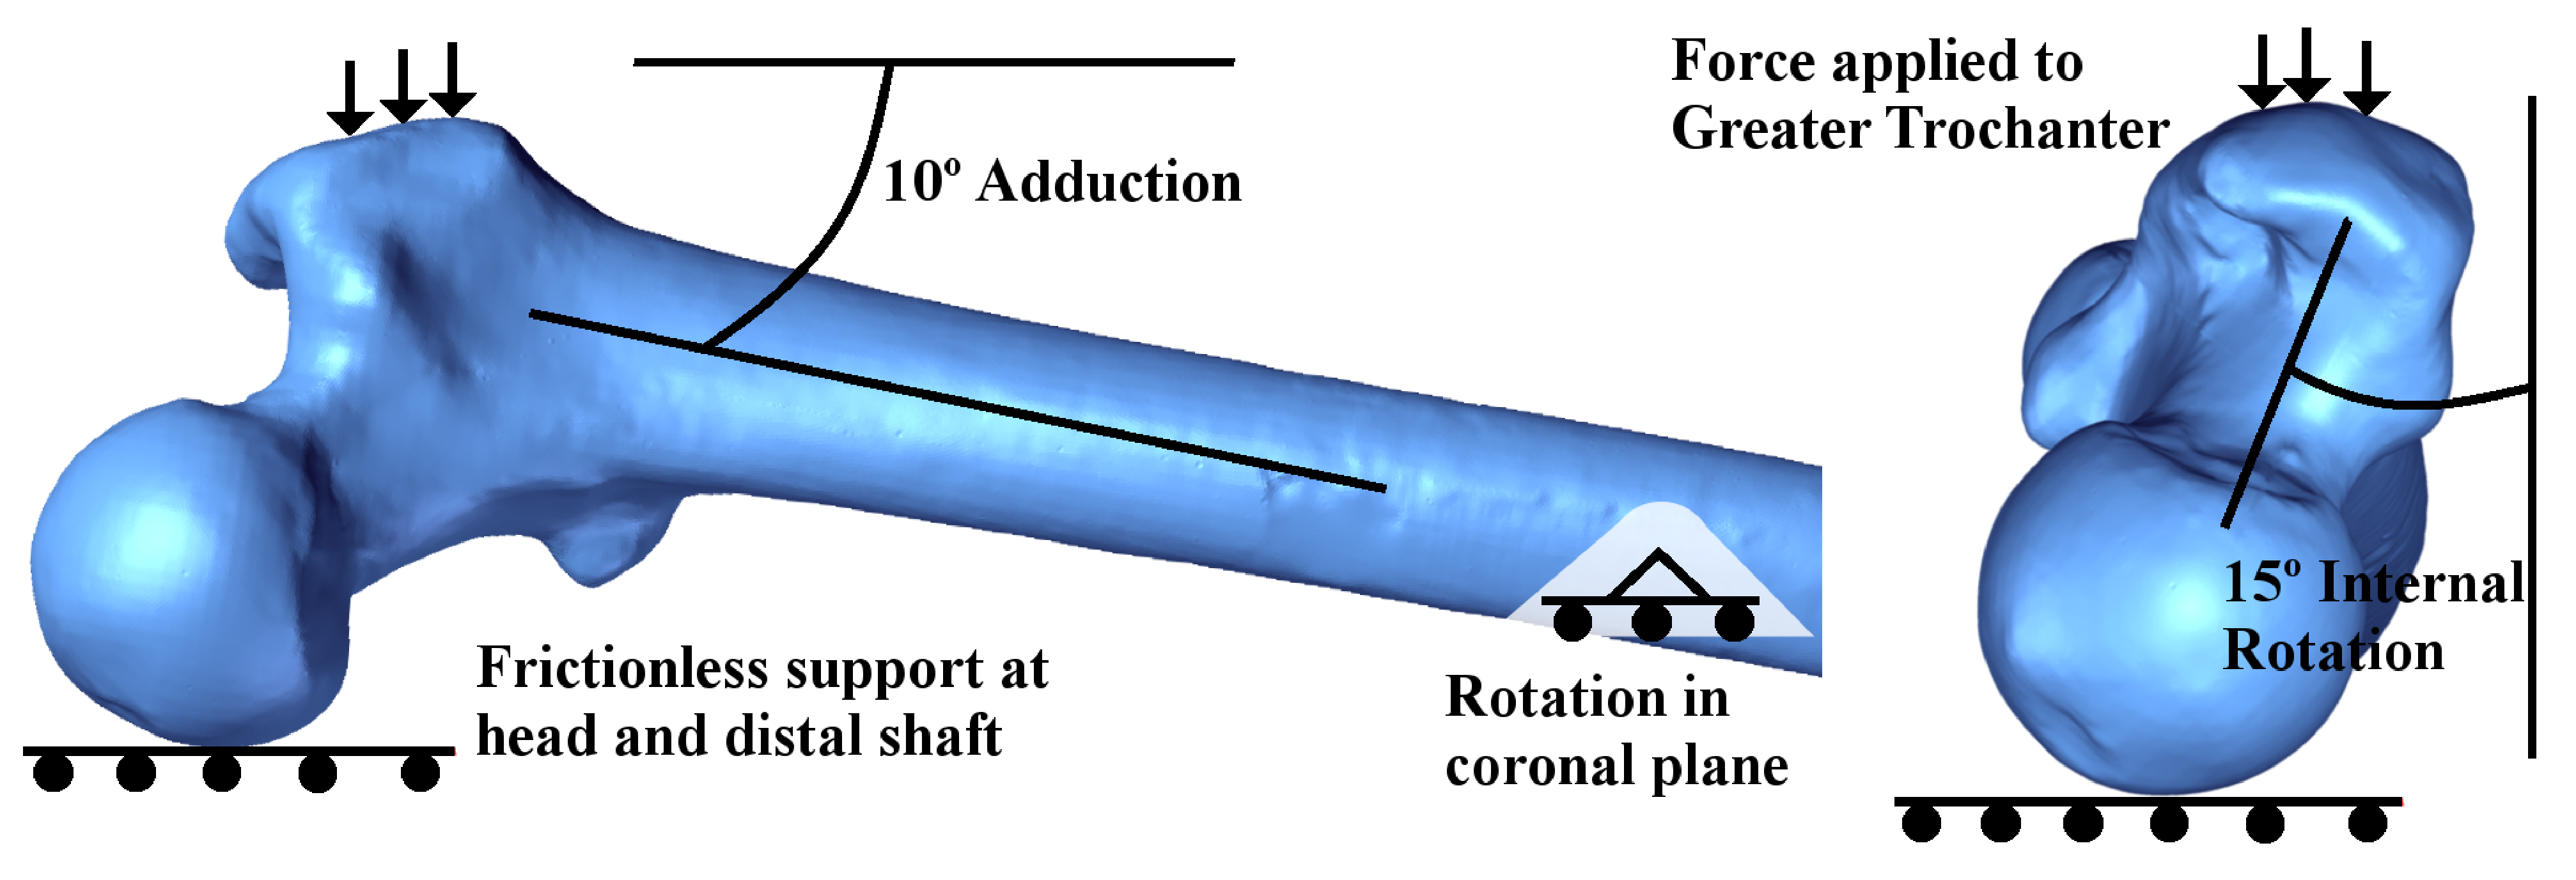
\includegraphics[width=1\linewidth]{./intro/Figures/FEM_Constraints}
	\caption[Proximal femur loading and orientation constraints]{\textbf{Constraints and orientation of the proximal femur in laboratory testing. Anterior view (left) and superior view (right).} Graphic \copyright Seth Gilchrist, 2013.}
	\label{fig:constraint_orient}
\end{figure}
	
\subsection{Application of force}
\label{sec:intro_understanding_modelling_lab_force}
The method used to apply force to the bone in a laboratory model can influence fracture because it changes loading and displacement rates.
The resulting loading and displacement rates could, in turn, affect the material properties due to the viscoelastic nature of bone, as discussed in~\S\ref{sec:intro_boneBehaviour}.
As the material in the bone fails, a progressive change in loading path and strain rates could then change the mechanics of the failure as discussed in~\S\ref{sec:intro_boneStrength}, such that erroneous force application could change the resulting failure and fracture patterns.

Force is applied to the lab models using either a constant displacement rate, or in some cases, an impact using a dropped mass.
\Citet{backman_proximal_1957} did not see any difference in fracture patterns between bones loaded at a constant compression rate and those loaded by impact.
Additionally, work examining bone tissue response to loading rate~\citep{carter_bone_1976, currey_effects_1975} showed a weak influence of strain rate to mechanical properties.
These two facts led early hip fracture researchers to use low, constant displacement rate at the greater trochanter~\citep{lotz_use_1990}.

Knowing that bone material is viscoelastic, researchers saw the application of the force using a low displacement rate as a possible weakness of the testing method, leading them to investigate the effects of increasing the displacement rates.
\Citet{courtney_effects_1994} used a materials testing machine to apply constant-rate displacements on donor-match pairs of femurs at 2~and 100~\ac{mm}/\ac{s}.
This work showed that increasing the displacement rate significantly increased the stiffness and energy to failure, and moderately increased the load to fracture.
In the years following this paper, many experiments have been carried out using a constant displacement rate of 100~\ac{mm}/\ac{s} at the greater trochanter~\citep{de_bakker_during_2009, manske_cortical_2008, manske_femoral_2006, sutter_biomechanical_2010}.
Displacement rate was not seen to influence positive correlation with \ac{abmd}, and results from lower rate tests are still considered valid.
Interestingly, the effects seen by \citet{courtney_effects_1994} were much stronger than would be predicted by isolated bone testing alone (\S\ref{sec:intro_boneBehaviour}).
If one assumes that the strain rate is directly proportional to displacement rate, one might expect an increase in displacement rate of 50x to increase the stiffness by approximately 20-30\%, and likely decrease the energy to failure~\citep{mcelhaney_dynamic_1966, carter_compressive_1977, linde_mechanical_1991}.
\Citet{courtney_effects_1994} found that femurs compressed at high displacement rates were approximately 100\% stiffer than those compressed at low rate and absorbed more energy to fracture, further illustrating the complexity in deriving organ level behaviours based on the behaviour of tissues.

Not all research has been conducted using constant velocity.
Three researchers~\citep{backman_proximal_1957, weber_proximal_1992, okuizumi_effect_1998} have utilized impacts to apply loads to specimens.
\citet{backman_proximal_1957} showed no difference in fracture pattern between impact and constant displacement rate loading.
However, his experiments were performed on dried femora and lacked the ability to accurately measure force or displacement, so were unable to evaluate biomechanical response to the different loadings.
\citet{weber_proximal_1992} used an impact at 4~\ac{m}/\ac{s} with an energy of 360~J (approximately 2-3x the current estimated energy in a fall to the side~\citep{robinovitch_distribution_1997, feldman_reducing_2007}) and found similar results to \citet{courtney_effects_1994}, in which all mechanical metrics increased as displacement rate increased.
\citet{okuizumi_effect_1998} investigated the effects of different hip protectors on the failure strength of proximal femurs using a dropped mass.
However, the impact mass, velocity and energy were not biomechanically justified and not compared to more traditional methods, so the influence of this protocol on the outcome is unknown.

\subsection{Lessons learned from laboratory models}
\label{sec:intro_understanding_modelling_lab_results}
As mentioned in \S\ref{sec:intro_understanding_tolerance}, once a laboratory model is validated for a certain scenario it can be used to examine any independent variable such as tissue displacement, force response, or yes/no injury classification.
Taking advantage of this aspect of laboratory models, many different properties of the proximal femur loaded in the fall configuration have been examined (Table \ref{tab:model_results}).

\let\thempfootnote\thefootnote
\def\arraystretch{1.5}

\begin{table}
\caption[Laboratory model results summary]{Important results and references for laboratory tests.}
\label{tab:model_results}
\begin{tabularx}{\textwidth}{l X p{4cm}}
\toprule
Aspect & Influence & Reference(s) \\ \midrule

Orientation & Increased internal rotation lowers ultimate strength. Standing vs.\ falling orientation changes strength, but ratio of the strengths depend on the definitions of ``standing" and ``falling". & \citep{pinilla_impact_1996, turner_biomechanics_2005, keyak_relationships_2000, lochmuller_mechanical_2002} \newline \citep{ford_effect_1996, keyak_effect_2001}\footnotemark  \\

Compression rate & Increased compression rate leads to increased stiffness, ultimate load and energy to failure. & \citep{courtney_effects_1994, weber_proximal_1992, okuizumi_effect_1998, backman_proximal_1957} \\

\ac{bmd} and \ac{abmd} & Higher \ac{bmd} leads to increased strength. & \citep{boehm_prediction_2008, bouxsein_ultrasound_1995, cheng_prediction_1998, cheng_assessment_1997, lochmuller_mechanical_2002, lotz_use_1990, roberts_comparison_2010, manske_cortical_2008, manske_femoral_2006, pulkkinen_experimental_2008, leichter_optical_2001} \\

Cancellous bone & Cancellous bone important in a fall, less so in standing. & \citep{manske_femoral_2006, manske_cortical_2008, holzer_hip_2009, pulkkinen_experimental_2008, blain_cortical_2008} \\

Cortical bone & Thin cortex is indicative of reduced strength. & \citep{lochmuller_mechanical_2002, manske_femoral_2006, manske_cortical_2008, crabtree_intracapsular_2001, de_bakker_during_2009, de_bakker_hip_2006, mayhew_relation_2005, blain_cortical_2008} \\

Age & Increased age relates to decreased \ac{bmd} and strength. & \citep{courtney_effects_1994, courtney_age-related_1995} \\

Side & Side-to-side strength in the same person differs on average by 19\% and 16\% for women and men, respectively. & \citep{eckstein_reproducibility_2004} \\

Geometry & Certain geometrical features, such as a long or narrow femoral neck, relate to increased fracture risk. & \citep{cheng_assessment_1997} \\

Failure location & Failure typically initiates in the anterior-superior neck. & \citep{de_bakker_hip_2006, de_bakker_during_2009} \\

Femoroplasty & Augmentation by femoroplasty (\ac{ie}, injection of bone cement to strengthen cancellous bone) increases strength of osteoporotic femurs, but makes revision surgery difficult or impossible. & \citep{heini_femoroplasty-augmentation_2004, beckmann_femoroplasty--augmentation_2007, sutter_biomechanical_2010, de_bakker_hip_2006} \\

\bottomrule
\end{tabularx}
\footnotetext[1]{Computational studies}
\end{table}

\def\arraystretch{1}

Orientation has been shown to influence femoral strength, with an increased internal rotation relating to a decrease in the strength of the specimen~\citep{pinilla_impact_1996, ford_effect_1996}.
Changing the orientation from a standing model to a side impact model showed a difference in one study~\citep{keyak_relationships_2000}, but not a second one~\citep{lochmuller_mechanical_2002}.
However, these two studies used different orientations to model a side impact, with~\citet{keyak_relationships_2000} using a rather extreme neck internal rotation of 70$^\circ$, which would be predicted to significantly lower the strength of the specimens~\citep{pinilla_impact_1996, ford_effect_1996, keyak_effect_2001, ford_effect_1996}.
	
\ac{bmd} has been included as a variable in many tests, and the data have consistently shown that a higher \ac{bmd} (or \ac{abmd}) leads to an increase in stiffness and ultimate load.

The independent roles of cancellous and cortical bone are known to some degree, but their relative roles are a bit more difficult to determine.
Cancellous bone has been shown to be important in a fall~\citep{manske_femoral_2006, manske_cortical_2008, pulkkinen_experimental_2008}, and less important in standing strength~\citep{holzer_hip_2009}.
Researchers who have compared the relative roles of cancellous and cortical bone in failure scenarios have shown that both have important roles to play, with relative importance varying by failure location~\citep{manske_cortical_2008, pulkkinen_experimental_2008}.

A decrease in strength of specimens loaded in a fall configuration has been shown to be correlated with increasing age; however that change was concurrent with a decrease in \ac{bmd}, which may have accounted for the decrease in strength~\citep{courtney_age-related_1995, courtney_effects_1994}.

Side-to-side strength in the same donor was seen to be  19~($\pm$13)\% (mean~($\pm$\ac{sd})) different in females and 16~($\pm$12)\% different in males~\citep{eckstein_reproducibility_2004}.
This result is important when considering the results of many of the comparative studies listed in Table \ref{tab:model_results}, because results from those studies were often analysed using matched-pairs statistics on donor-matched pairs of femurs.
\citet{eckstein_reproducibility_2004} showed that matched-pairs statistics on donor-matched (left \ac{vs} right) femurs is likely insufficient for statistical significance, as there is considerable variability in strength that is unexplained by \ac{bmd}.

Geometry has been thought to be a promising clinical screening tool, as it can be evaluated using planar x-rays.
As such, it has been predominately studied using clinical methods~\citep{dincel_association_2008, el-kaissi_femoral_2005, faulkner_simple_1993, wang_women_2009}.
Femoral neck length, measured from the medial head to the lateral cortex of the greater trochanter, shows the highest correlation with fracture load~\citep{cheng_assessment_1997}, however this correlation is much lower than that of \ac{bmd} with fracture load.
Clinical evaluations showed that femoral neck length, and hip axis length (which is defined as the distance from the medial border of the pelvis, adjacent to the acetabulum, to the lateral cortex of the greater trochanter along the femoral neck) both correlate with hip fracture risk, but are most powerful when used in conjunction with \ac{bmd}~\citep{faulkner_simple_1993, dincel_association_2008}.

Failure location has been experimentally confirmed in only one study~\citep{de_bakker_during_2009} (and an associated thesis~\citep{de_bakker_hip_2006}).
Fractures were seen to typically originate in the superior or anterior femoral neck, regardless of fracture type (\ac{eg}, cervical or trochanteric).
That said, trochanteric fractures appeared to originated in the lateral neck, whereas neck fractures originated in the sub-capital region.

Femoroplasty is a technique in which \ac{pmma} (\ac{aka}\ bone cement) is injected into the proximal femur as a way to reinforce the senile trabecular structure.
Studies on femoroplasty have shown that it significantly increases strength and energy to failure~\citep{de_bakker_hip_2006, heini_femoroplasty-augmentation_2004, sutter_biomechanical_2010}.
These benefits are currently outweighed by complications in dealing with large quantities of \ac{pmma}, which include the highly exothermic reaction as it sets~\citep{de_bakker_hip_2006, heini_femoroplasty-augmentation_2004}, and difficulty with revision surgery due to the hardness of the material~\citep{beckmann_femoroplasty--augmentation_2007}.
	
\subsection{Limitations of laboratory models}
\label{sec:intro_understanding_modelling_lab_limits}
The data gathered in laboratory experiments are of great importance to an understanding how the proximal femur behaves during a fall to the side.
However, there are limitations to the current laboratory models which must be understood in order to apply the results.
One of the principal limitations is the lack of a biofidelic, dynamic model of the fall.
Previously published models attempt to apply loads representative of a fall by applying a constant-rate compression of 100~\ac{mm}/\ac{s}.
This compression rate has never been validated as a reasonable value, and therefore must be taken with caution -- especially given the influence it has on the behaviour of the bone.

The majority of the models use materials testing machines to apply compression to the lateral trochanter, and continue compression until fracture is attained.
This method of creating fractures ignores the fact that the bone is not loaded in constant displacement rate.
Rather, it is loaded by the inertia of a falling mass (\ac{ie}, the body) and mediated by deformable elements (\ac{eg}, pelvis, skin and fat).
This means that the loading conditions (such as displacement rate) will be a function of the fall characteristics and the properties of the proximal femur itself. 
Additionally, the energy of the mass in the fall is limited and fracture is not guaranteed.
In fact, fracture is seen in only $\sim$5\% of real-world falls in the elderly~\citep{masud_epidemiology_2001, nachreiner_circumstances_2007}.

The results of the laboratory models are also at odds with the epidemiology.
Laboratory fracture models have failed to identify any significant predictor of fracture besides \ac{bmd}.
Studies of fractures in the general population show a considerable overlap of \acp{bmd} between fracture and non-fracture patients~\citep{greenspan_fall_1994, faulkner_simple_1993}.
As few as 22\% of hip fractures patients have \acp{bmd} that would classify as osteoporotic, and 42\% that would classify as osteopenic or osteoporotic~\citep{stone_bmd_2003}.
This could be due to the use of ultimate load as the criteria for fracture resilience, and also may be influenced by the constant displacement rate, rather than inertial impact, testing method.		

\subsection{Summary}
\label{sec:intro_understanding_modelling_lab_summary}
Laboratory models of hip fracture have been used extensively to determine the influence of different aspects of the proximal femur on its strength.
The primary focus of the modelling has been to understand the strength in a fall to the side, and in this respect researchers have developed methods that have shown the influence of many physical characteristics.
Even with all of this effort and knowledge, there are still gaps between what is being modelled and the real world.
A potential next step in laboratory testing is to refine the model of a fall to the side, increasing its biofidelity to allow researchers to understand the inputs and results of real world falls.

\section{Computer models}
\label{sec:intro_understanding_modelling_comp}
Computer models are performed using the \acf{fe} and \acf{mbd} techniques.
Most of the information about the mechanism of hip fracture gleaned from computer models has come from \ac{fe} models because they are capable of providing stresses, strains and potential failure locations.
This section focuses on the contributions and limitations of \ac{fe} models.
There have been few \ac{mbd} models that have provided insight into hip fracture, focusing primarily on determining the fall conditions, which are discussed more thoroughly in Chapter \ref{ch:fall_sim_design}.

\subsection{Contributions of \acs*{fe} models}
\label{sec:intro_understanding_modelling_comp_use}
\ac{fe} models are, in most cases, based on a laboratory model that can be used as a validation.
Once an \ac{fe} model is validated, it can be used to examine a number of different aspects of the failure event, including the role of soft tissue~\citep{majumder_simulation_2007}, fall modelling~\citep{majumder_effects_2008}, non-invasive strength estimation for an arbitrary bone~\citep{keaveny_femoral_2008, srinivasan_relationship_2011, viceconti_automatic_2004}, and fracture risk estimation~\citep{orwoll_finite_2009, srinivasan_relationship_2011, tanck_predictive_2009}.

In addition to all of these uses, \ac{fe} models have been used to understand the fracture itself.
Multiple researchers have used \ac{fe} models to estimate the location where fractures begin and what conditions lead to fracture~\citep{keyak_prediction_2001, keyak_prediction_2000, keyak_prediction_1998, nawathe_microstructural_2013, lotz_fracture_1991, lotz_fracture_1991-1, lotz_stress_1995, ota_fracture_1999, tanck_predictive_2009, verhulp_comparison_2006, verhulp_load_2008, bryan_use_2009}.
Data from these models have increased the understanding of the conditions in the femur leading up to fracture, but there are significant limitations to the models that can affect interpretation of their results.
	
\subsection{Limitations of \acs*{fe} models}
A primary limitation of \ac{fe} models relates to the experimental models used to determine their validity.
As discussed in \S\ref{sec:intro_understanding_modelling_lab}, the displacement rate used to load a proximal femur can influence its mechanical and failure behaviours.
It is thought that these changes in organ level behaviour originate from changes at the bone material level (see~\S\ref{sec:intro_boneBehaviour} and~\S\ref{sec:intro_boneStrength}).
The experiment used to validate an \ac{fe} model should replicate the boundary and loading conditions applied in the model, and also have the similar material properties as those applied in the model.
Failing to meet these requirements can lead to validation uncertainty.

The material properties applied to a model are often determined from tissue level tests conducted at low strain rate, while the validation experiment is an organ level test conducted at high displacement rate (\ac{eg}, 100~mm/s).
As a result, it is possible that significant differences exist in bone properties in the tissue and organ level tests.
If the \ac{fe} model agrees with the organ level test, it could be due to an error in the model (such as an inappropriate constraint), rather than accurate representation of the experiment.

It is possible that the displacement rate does not affect the desired outcome variable, making the selection of a validation experiment essentially arbitrary.
However, if there is a dependence on experimental method, \ac{fe} researchers must be sure to select material properties that are in agreement with their validation experiments.
Currently, there is no standard for what experiment should be used to validate a given \ac{fe} outcome variable and therefore special attention should be paid to possible interplay between materials definitions and model validation.

In addition to validation challenges, selecting appropriate material properties for the \ac{fe} model can be complicated.
As we have seen in previous sections, bone is a highly complex material at all length scales, making simplifications for computational applications necessary.
The majority of \ac{fe} models use relatively simple material definitions that lack the anisotropy and viscoelasticity discussed in \S\ref{sec:intro_boneBehaviour}.
This lack of fidelity in the material model may influence how load is transferred and how failure is determined given that ultimate strain is a function of strain rate.
Additionally, they use a single phase, neglecting the flow of bone marrow, which has been shown to be important at high strain rates~\citep{carter_compressive_1977}.
A final limitation of the material definitions in current \ac{fe} models is the use of a highly simplified post yield behaviour model.
After yield, bone behaviour is dependent on the bone type~\citep{hayes_biomechanics_1997}, loading direction~\citep{hansen_effect_2008}, and loading rate~\citep{hansen_effect_2008, kulin_effects_2011, kulin_loading_2011}, making computational modelling very difficult.
There are efforts to address this final limitation using plastic material models for post yield behaviour~\citep{derikx_implementation_2011, verhulp_micro-finite_2008, bayraktar_comparison_2004}.
However, those models are still simple, modelling both tension and compression in the same manner, and lacking the non-linearity of post-yield strain with strain rate seen in the bone core tests described in \S\ref{sec:intro_boneStrength}~\citep{derikx_implementation_2011, bayraktar_comparison_2004}.

Another limitation of \ac{fe} models of biological systems is that they are deterministic in nature, \ac{ie}, each model has only one solution, even though there are many probable outcomes for a given loading scenario in the physiological situation.
This limitation has been addressed using Monte Carlo simulations for material and geometry, which provide a distribution of strains or stresses for a given element, in a given loading scenario~\citep{bryan_use_2009, taddei_finite-element_2006, laz_incorporating_2007}.
These statistical simulations attempt to address the uncertainly regarding material properties and geometry, but do not address uncertainly in fluid flow, or changes in material properties due to deformation, strain rate, or loading direction.
	
One final but important note relating to the interpretation of the results of \ac{fe} models is that many predict failure in the cancellous bone~\citep{bryan_use_2009, keyak_prediction_2001, keyak_prediction_2000, keyak_prediction_1998, lotz_fracture_1991, lotz_stress_1995, nawathe_microstructural_2013, verhulp_comparison_2006, verhulp_load_2008}.
This result is intriguing, but one must remember computational models are only valid for output variables that have been validated.
Since the deformation of the cancellous bone cannot be directly measured in experimental tests, it has never been validated, and this necessarily limits the scientific reliability of these data.
To fully trust the results that are given for internal strains, a method needs to be devised and implemented to experimentally determine the actual internal deformations for comparison and validation.

\subsection{Applications of models to fracture prevention}
\label{sec:intro_understanding_application}
Modelling results have been applied to the development of a number of different biomechanical technologies that are intended to prevent hip fracture.
The most advanced in terms of development and assessment are hip protectors, which are soft or hard pads that are positioned over the greater trochanters using special undergarments.
Hip protectors have been shown to decrease the impact force~\citep{choi_effect_2010,laing_force_2008, van_schoor_biomechanical_2006}, but have not proven effective in the real-world~\citep{kiel_efficacy_2007, parker_effectiveness_2006}.

Another more recent development is compliant flooring, which modifies the landing surface in order to decrease the impact force~\citep{laing_effect_2006, li_comparison_2013}.
This technology is currently in the development and proving stage~\citep{clinicaltrials.gov_flooring_2012}, but shows promise as a passive strategy to protect individuals against fracture in a way that is effective immediately and not compromised by lack of compliance -- the two main problems with pharmacological remedies (which can take years to become effective) and hip protectors (which are often not worn at the time of a fracture).

Both of these technologies use data from modelling of hip fracture to determine the target maximum forces in their simulated falls.
Some tests also use knowledge of where fractures are likely to occur to determine effectiveness for a particular injury~\citep{laing_force_2008}.

\chapter{Objective and research questions}
\label{sec:intro_goals}
The objective of this thesis is to quantitatively compare the mechanical and failure behaviours of hip fracture in constant displacement rate loading with the behaviours in impact fall simulation.
Specifically, this research will determine if experimental constant displacement rate models of hip fracture produce force-displacement, strain, failure and fracture results that are similar to those observed in impact fall simulation.
Any differences observed in the behaviours of the bones between these two experimental models will inform a decision matrix.
This matrix can be used as a guide by \textit{ex vivo} and \ac{fe} modellers to select the most appropriate experiment for their outcome variables or validation needs.

\section{Research questions}
\label{sec:intro_goals_questions}
In pursuit of these objectives, I have identified three research questions:
\begin{enumerate}
\item Does the force-displacement mechanical response of a proximal femur differ when it is loaded using constant displacement rates \ac{vs} impact fall simulation?
\item Does the surface strain field of the proximal femur differ when it is loaded using constant displacement rates \ac{vs} impact fall simulation?
\item Do the locations of initial failure and final fracture change when the proximal femur is loaded using constant displacement rates \ac{vs} impact fall simulation?
\end{enumerate}

\section{Method of investigation}
\label{sec:intro_method}
To answer the research questions, an inertially driven fall simulator with elements modelling the body, pelvis, and soft tissues over the greater trochanter has been built.
Its design and development are discussed in Chapter \ref{ch:fall_sim_design}.
This fall simulator was used in conjunction with a materials testing machine to determine if the mechanical, strain and failure  behaviours of the proximal femur are similar or divergent between the quasi-static and impact loading methods.

\subsection[Force-displacement behaviour]{Does the force-displacement behaviour differ between constant displacement rate and impact fall simulation testing?}
\label{sec:intro_method_behave}
This question was addressed by comparing the sub-failure, force-displacement response of proximal femurs loaded using quasi-static, constant displacement rates in a materials testing machine and the response of the same femurs loaded to failure in the impact fall simulator.
Single specimens were loaded to 50\% of their \ac{abmd} predicted failure load in a materials testing machine, and the behavioural metrics of force, displacement, stiffness, and energy to maximum applied load were measured.
The same bones were then transferred to the impact fall simulator and loaded to failure.
The same metrics measured in the quasi-static tests were measured in the fall simulation tests and compared to the quasi-static results at the the maximum load applied in the materials testing machine.
This research is presented in Chapter~\ref{ch:behave_fail}.

\subsection[Strain behaviour]{Does the surface strain differ between constant displacement rate and impact fall simulation testing?}
\label{sec:intro_method_fail}
This question was addressed using stereo \acf{dic} of the anterior-superior surface of the femoral neck. % during quasi-static, constant displacement rate loading in a materials testing machine and impact fall simulation.
Stereo, \ac{3d} \ac{dic} data were collected on the anterior-superior femoral neck of single specimens loaded to 50\% of their \ac{abmd} predicted failure loads in a materials testing machine, followed by loading to failure in the impact fall simulator.
The \ac{3d} surface profiles measured by the \ac{dic} software were aligned, and the minimum principal strains on the surfaces were compared to determine if there was a difference in strain magnitude or distribution between the two loading protocols.
This work is presented in Chapter~\ref{ch:fracture}.

\subsection[Failure behaviour]{Do the failure locations and final fracture types differ between constant displacement rate and impact fall simulation testing?}
\label{sec:intro_method_fracture}
This question was addressed using two groups of specimens, one group loaded to failure in a materials testing machine under quasi-static, constant displacement rates and another group loaded to failure in the impact fall simulator.
Fracture locations were determined from high-speed videos of the experiments and final fracture types were classified by an orthopaedic surgeon and compared between the two groups.
This research is presented in Chapter~\ref{ch:fracture}.